\apendice{Documentación de usuario}

\section{Introducción}

En este anexo se pretende describir de forma concisa las características y funcionalidades de la \textit{web} desarrollada, además de los requisitos necesarios para su correcta renderización.

Es importante destacar que la \textit{web} ha sido desplegada en Heroku. Sin embargo, esta PaaS, tiene importantes restricciones en las versiones para estudiantes. En concreto, Krini se ve gravemente perjudicada ya que Heroku cancela toda petición que dure más de 30 segundos (lo que impide, en la mayoría de los enlaces, realizar un análisis completo).

Por este motivo, también se va a documentar cómo desplegar la aplicación en local (servidor de producción y base de datos) mediante contenedores de Docker.

\section{Requisitos de usuarios}

En este apartado se pretenden enumerar los requisitos necesarios para acceder correctamente a la \textit{web} desarrollada.

\subsection{Requisitos Heroku}
\label{s-e:requisitos-heroku}

Los requisitos en este caso vienen limitados por el uso de las bibliotecas \texttt{Chart.js} (v2.9.3) y \texttt{Bootstrap} (v4.4.1). En este caso, se necesita que la \textit{web} se renderice en navegadores con las siguientes versiones:

\begin{itemize}
	\item \textbf{Google Chrome:} todas las versiones modernas.
	\item \textbf{Mozilla Firefox:} todas las versiones modernas.
	\item \textbf{Safari:} todas las versiones modernas.
	\item \textbf{Microsoft Edge:} todas las versiones modernas.
	\item \textbf{Internet Explorer:} versión 10 o superior.
\end{itemize}

\subsection{Requisitos Docker}
\label{s-e:requisitos-docker}

Además de los requisitos expuestos en la sección~\ref{s-e:requisitos-heroku}, si se quiere ejecutar el contenedor de Docker en local, se ha de cumplir con las siguientes características en función del sistema operativo. Es relevante que, como se puede comprobar en el diagrama de despliegue de Docker (disponible en la ilustración~\ref{c:diagrama-deploy-docker}), los contenedores de la base de datos y de la \textit{web} son independientes. Por ello, se ha de contar con el \textit{plugin} \texttt{docker-compose}.

\begin{enumerate}
	\item \textbf{Windows}: se recomienda utilizar Docker Desktop por su simplicidad. Los requisitos completos se pueden consultar en su documentación oficial\footnote{Disponible en \url{https://docs.docker.com/desktop/install/windows-install/}}. Sin embargo, se resumen a continuación:
	
	\begin{itemize}
		\item \texttt{WLS}
		\item Procesador de 64 bits
		\item 4GB de memoria RAM
		\item 3GB de memoria para las imágenes
		\item El \textit{plugin} \texttt{docker-compose} viene por defecto con la versión de escritorio.
	\end{itemize}

	\item \textbf{Linux}: nuevamente, los requisitos completos se facilitan en la documentación\footnote{Disponible en \url{https://docs.docker.com/desktop/install/linux-install/}}. En resumen, se recomienda:
	\begin{itemize}
		\item Disponer de soporte para virtualización
		\item Procesador de 64 bits
		\item 4GB de memoria RAM
		\item 3GB de memoria para las imágenes
		\item Instalar el \textit{plugin} \texttt{docker-compose} mediante \texttt{\$ sudo apt-get install docker-compose-plugin} (en Ubuntu y Debian) o \texttt{\$ sudo yum install docker-compose-plugin} (en distribuciones basadas en RPM).
	\end{itemize}
\end{enumerate}



\section{Instalación}

La instalación de un producto \textit{software} es el proceso mediante el cual se configura y prepara un programa o aplicación para que pueda ser utilizado en un dispositivo objetivo.

Debido a que la aplicación desarrollada es una \textit{web}, no hace falta pasar por este proceso. Sin embargo y debido a las restricciones de Heroku anteriormente mencionadas, se va a explicar cómo desplegar la aplicación en local mediante Docker (con servidores de producción) para comprobar la funcionalidad al completo. Se recuerda que las instrucciones para levantar el servidor de desarrollo se encuentran en la sección~\ref{s-d:flask-deploy}.

\subsection{Acceso mediante Heroku}

Simplemente se ha de acceder mediante el navegador introduciendo la dirección \url{https://krini.herokuapp.com/}

\subsection{Despliegue en Docker}
\label{s-e:docker-deploy-users}

Para facilitar que cualquier usuario pueda desplegar un contenedor de Docker (en realidad, dos) y levantar su propio servidor de gunicorn en local sin tener conocimientos técnicos, se han preparado unos \textit{scripts} multiplataforma disponibles en \url{https://github.com/phf1001/semisupervised-learning-in-cibersecurity/tree/main/docker-deploy-kit}

De esta forma, tan solo se debe seleccionar el sistema operativo anfitrión, descargar los archivos (se facilita un comprimido con todos incluidos) y garantizar que se cumple con los requisitos de la sección~\ref{s-e:requisitos-docker}.

Para levantar el servidor en local y garantizar que la base de datos se rellena completamente, se han de seguir los siguientes pasos teniendo en cuenta que los \textit{scripts} en Linux se ejecutan mediante el comando \texttt{\$ sh nombre-script.sh} y en Windows mediante \texttt{\$ nombre-script.bat}.

\begin{enumerate}
	\item Ubicarse en la carpeta donde se encuentren los \textit{scripts}.
	\item Si es la primera vez que se ejecuta:
	\begin{enumerate}
	\item Lanzar el script \texttt{docker-first-time-1.sh} y seguir las instrucciones (esperar 30 segundos y abrir el navegador cuando lo indique).
	\item Ejecutar el \textit{script} \texttt{docker-first-time-2.sh} y respetar los pasos indicados (esperar 30 segundos antes de abrir el navegador).
	\end{enumerate}
	\item Si se quieren parar los contenedores para reutilizarlos luego, ejecutar el \textit{script} \texttt{docker-stop.sh} y \texttt{docker-start.sh} para volver a iniciarlos.
	\item Si se quieren borrar las imágenes y contenedores del sistema definitivamente, ejecutar el \textit{script} \texttt{docker-clean.sh}
\end{enumerate}

\textbf{Importante}: iniciar el demonio de Docker antes de lanzar los \textit{scripts}. En Windows basta con ejecutar la aplicación de escritorio.

\section{Manual del usuario}

En este punto del manual se supone que todos los usuarios tienen acceso a la aplicación, ya sea mediante un contenedor de Docker o Heroku.

A continuación, se procede a ilustrar las funcionalidades básicas de la \textit{web}. Es destacable que no todos los usuarios cuentan con acceso a todas las funcionalidades (consultar diagrama de casos de uso~\ref{b:diagrama-cu}). Por ello, se recomienda probar el producto con una cuenta con permisos de administración.


\subsection{Analizador}
\label{s-e:analizador}

\begin{figure}[h]
	\caption[Manual de usuario: página principal]{Página principal de la aplicación.}
	\centering
	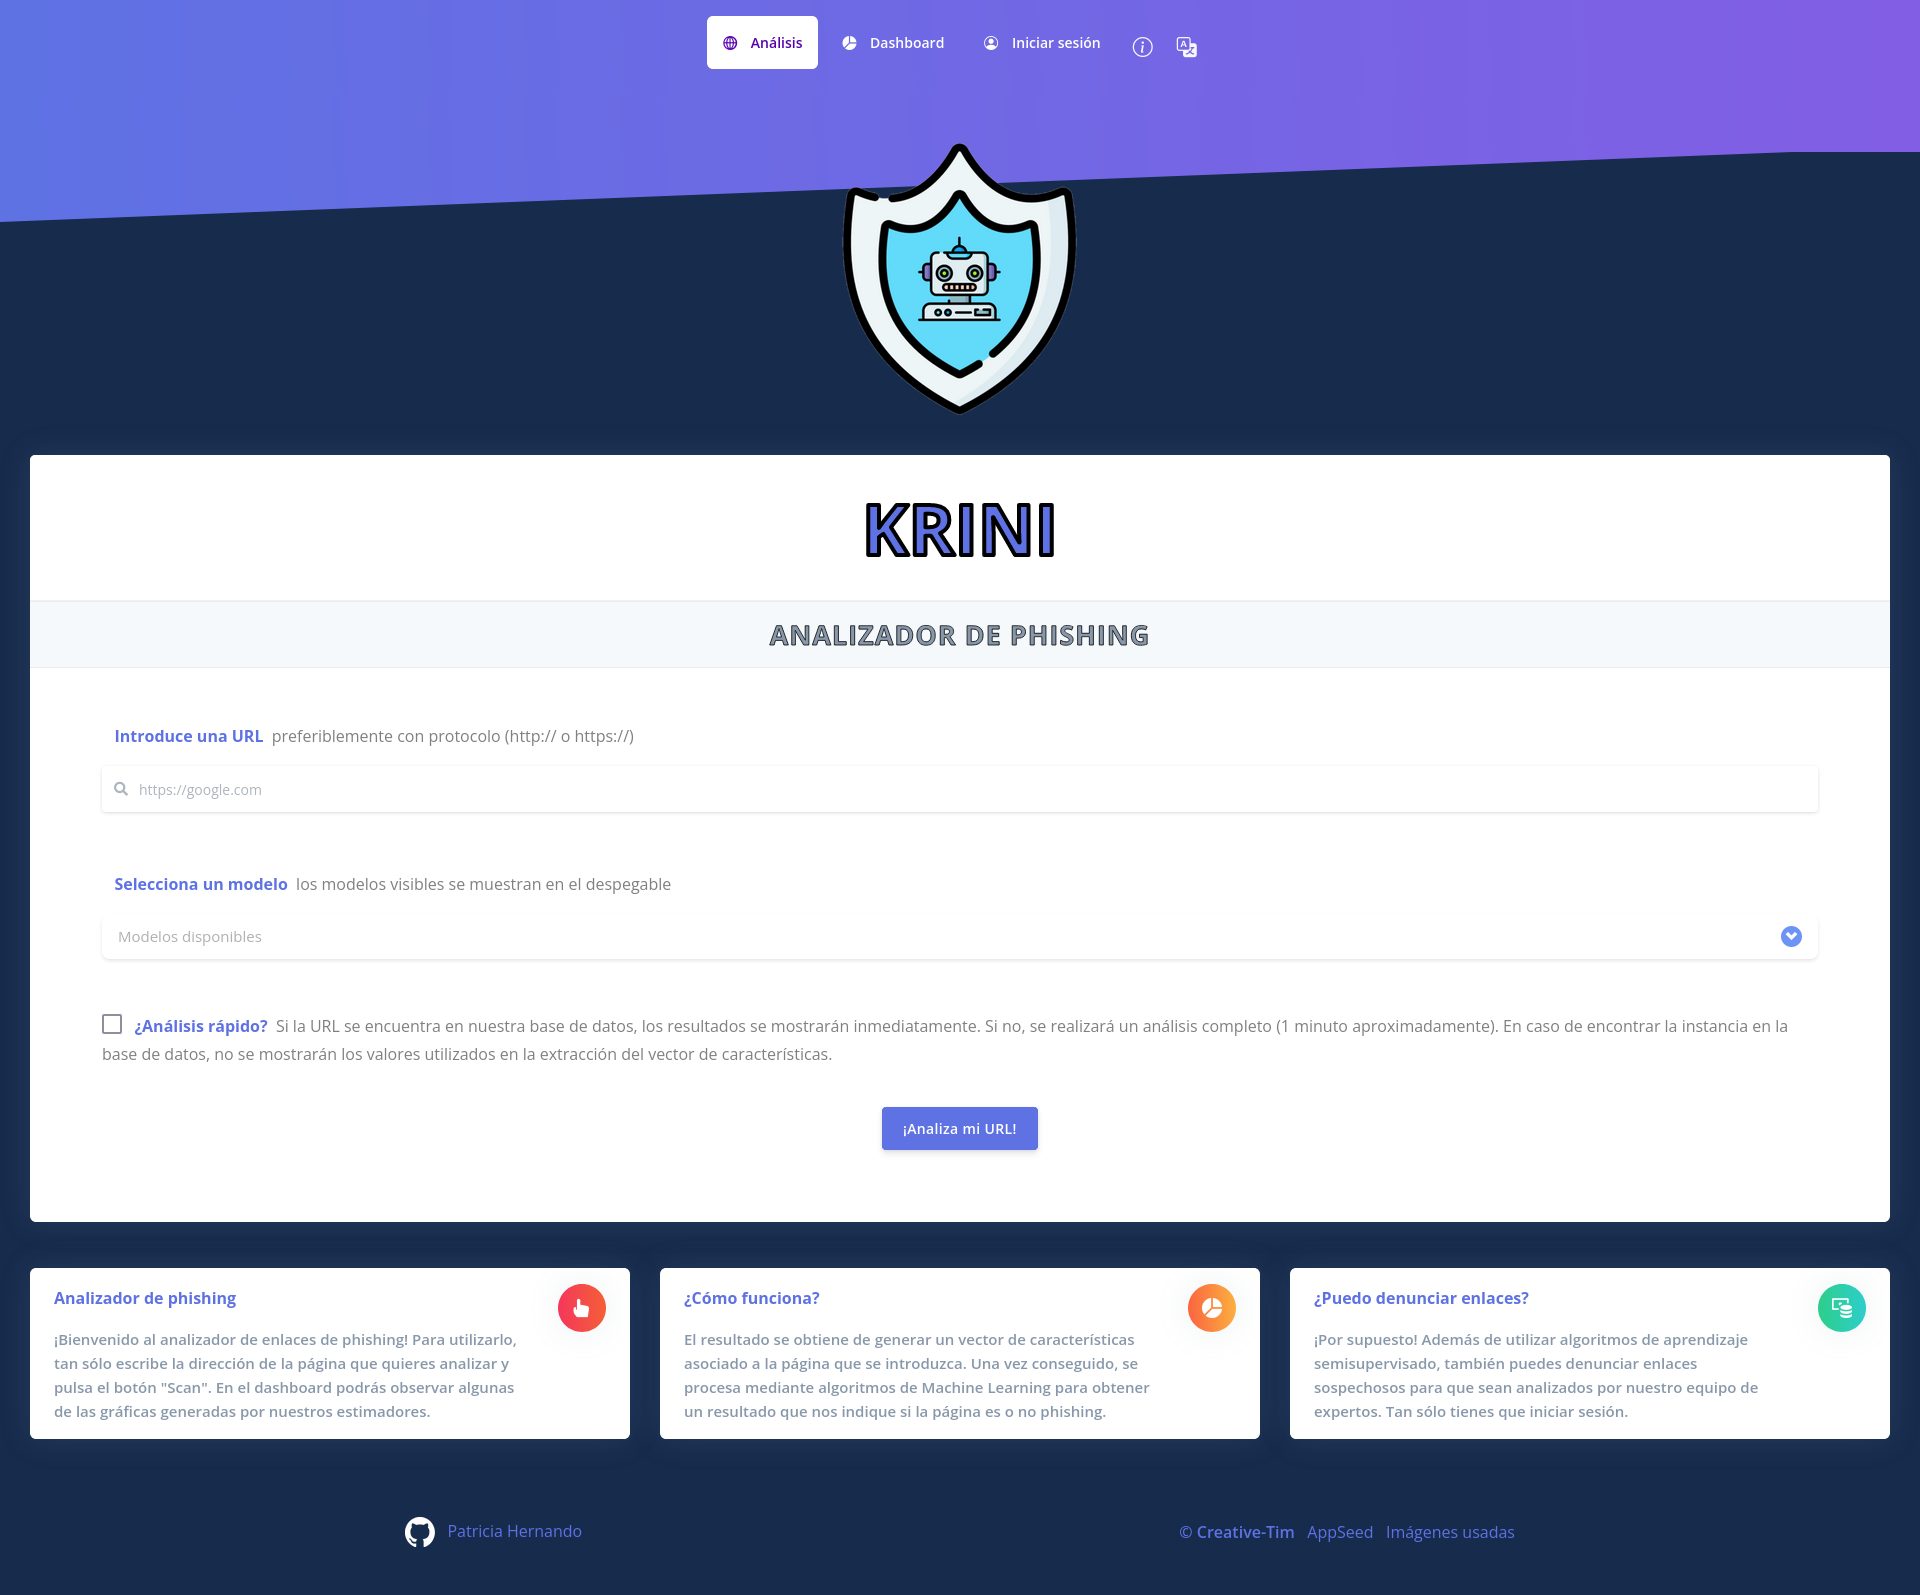
\includegraphics[width=\textwidth]{../img/anexos/user_guide/1_index}
	\label{e-1:index}
\end{figure}

En la ilustración~\ref{e-1:index} se muestra la página principal del analizador disponible para cualquier usuario. Para escanear una URL, basta con introducirla en el campo correspondiente. Es preferible introducir la dirección tal y como aparece en el navegador, pero si no es posible, la aplicación tratará de autocompletarla.

A continuación se pueden seleccionar los clasificadores que se deseen en el desplegable. Si no se selecciona ninguno, se analizará con el modelo por defecto, y en caso de que no exista, con uno aleatorio.

Opcionalmente se puede marcar la casilla <<análisis rápido>>. En este caso, no se extraerá el vector de características si ya existe en la base de datos\footnote{Para garantizar que la base de datos se autocompleta, cualquier vector de características nuevo que se extraiga por un usuario registrado se guardará en la sección de <<instancias>> (consultar sección~\ref{s-e:instances} del manual) con etiquetas adecuadas (\texttt{new-instance}, \texttt{auto-classified} y \texttt{recommendation-review}) y se incluirá una sugerencia para su revisión (\texttt{suggestion-review-new-scanned}).}.
 
Tras pulsar el botón de analizar, se mostrará una pantalla de carga mientras se extrae el vector de características correspondiente a la URL introducida (imagen~\ref{e-1:analysis}). En caso de error, se volverá a la página principal con un mensaje informativo.

\begin{figure}[h]
	\caption[Manual de usuario: página de carga]{Página de análisis de URL.}
	\centering
	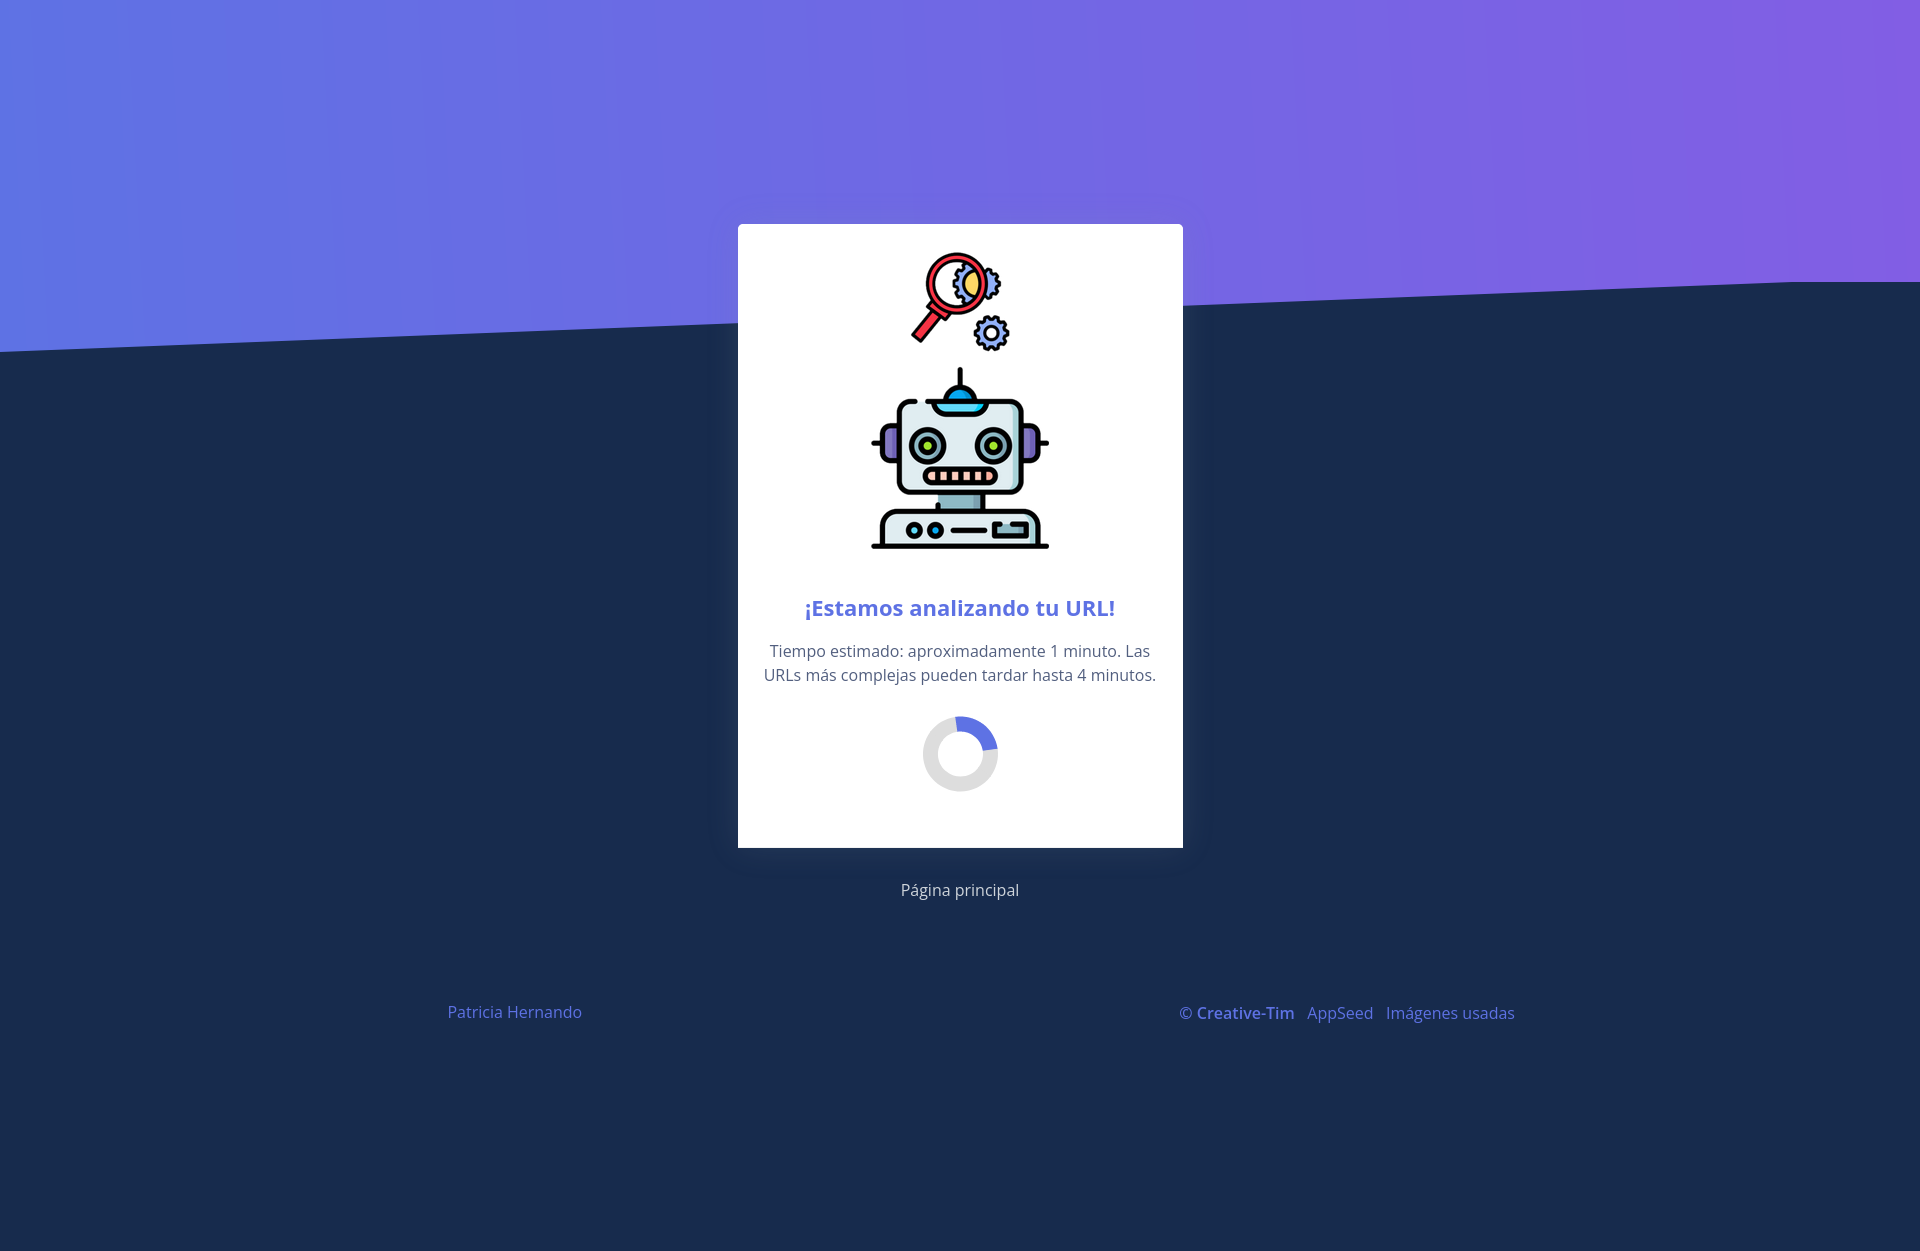
\includegraphics[width=\textwidth]{../img/anexos/user_guide/2_analysis}
	\label{e-1:analysis}
\end{figure}

\subsection{\textit{Dashboard}}
\label{s-e:dashboard}

En el \textit{dashboard} se pueden observar los resultados de analizar la URL introducida mediante los clasificadores seleccionados.

Las gráficas interactivas (imagen~\ref{e-3:dashboard-1}) se muestran tanto si se ha realizado un análisis rápido como si no. En un primer lugar se realiza una comparativa entre clasificadores. A continuación, se representa en un gráfico de tipo \textit{doughnut} las predicciones de todos los estimadores y en una tabla la seguridad de cada clasificador en la predicción. Por último, se pueden contemplar individualmente las estadísticas de cada clasificador en la gráfica giratoria (pulsar el botón <<siguiente>> para cambiar entre gráficas).

\begin{figure}[h]
	\caption[Manual de usuario: gráficas del \textit{dashboard}]{\textit{Dashboard} mostrado tras un análisis.}
	\centering
	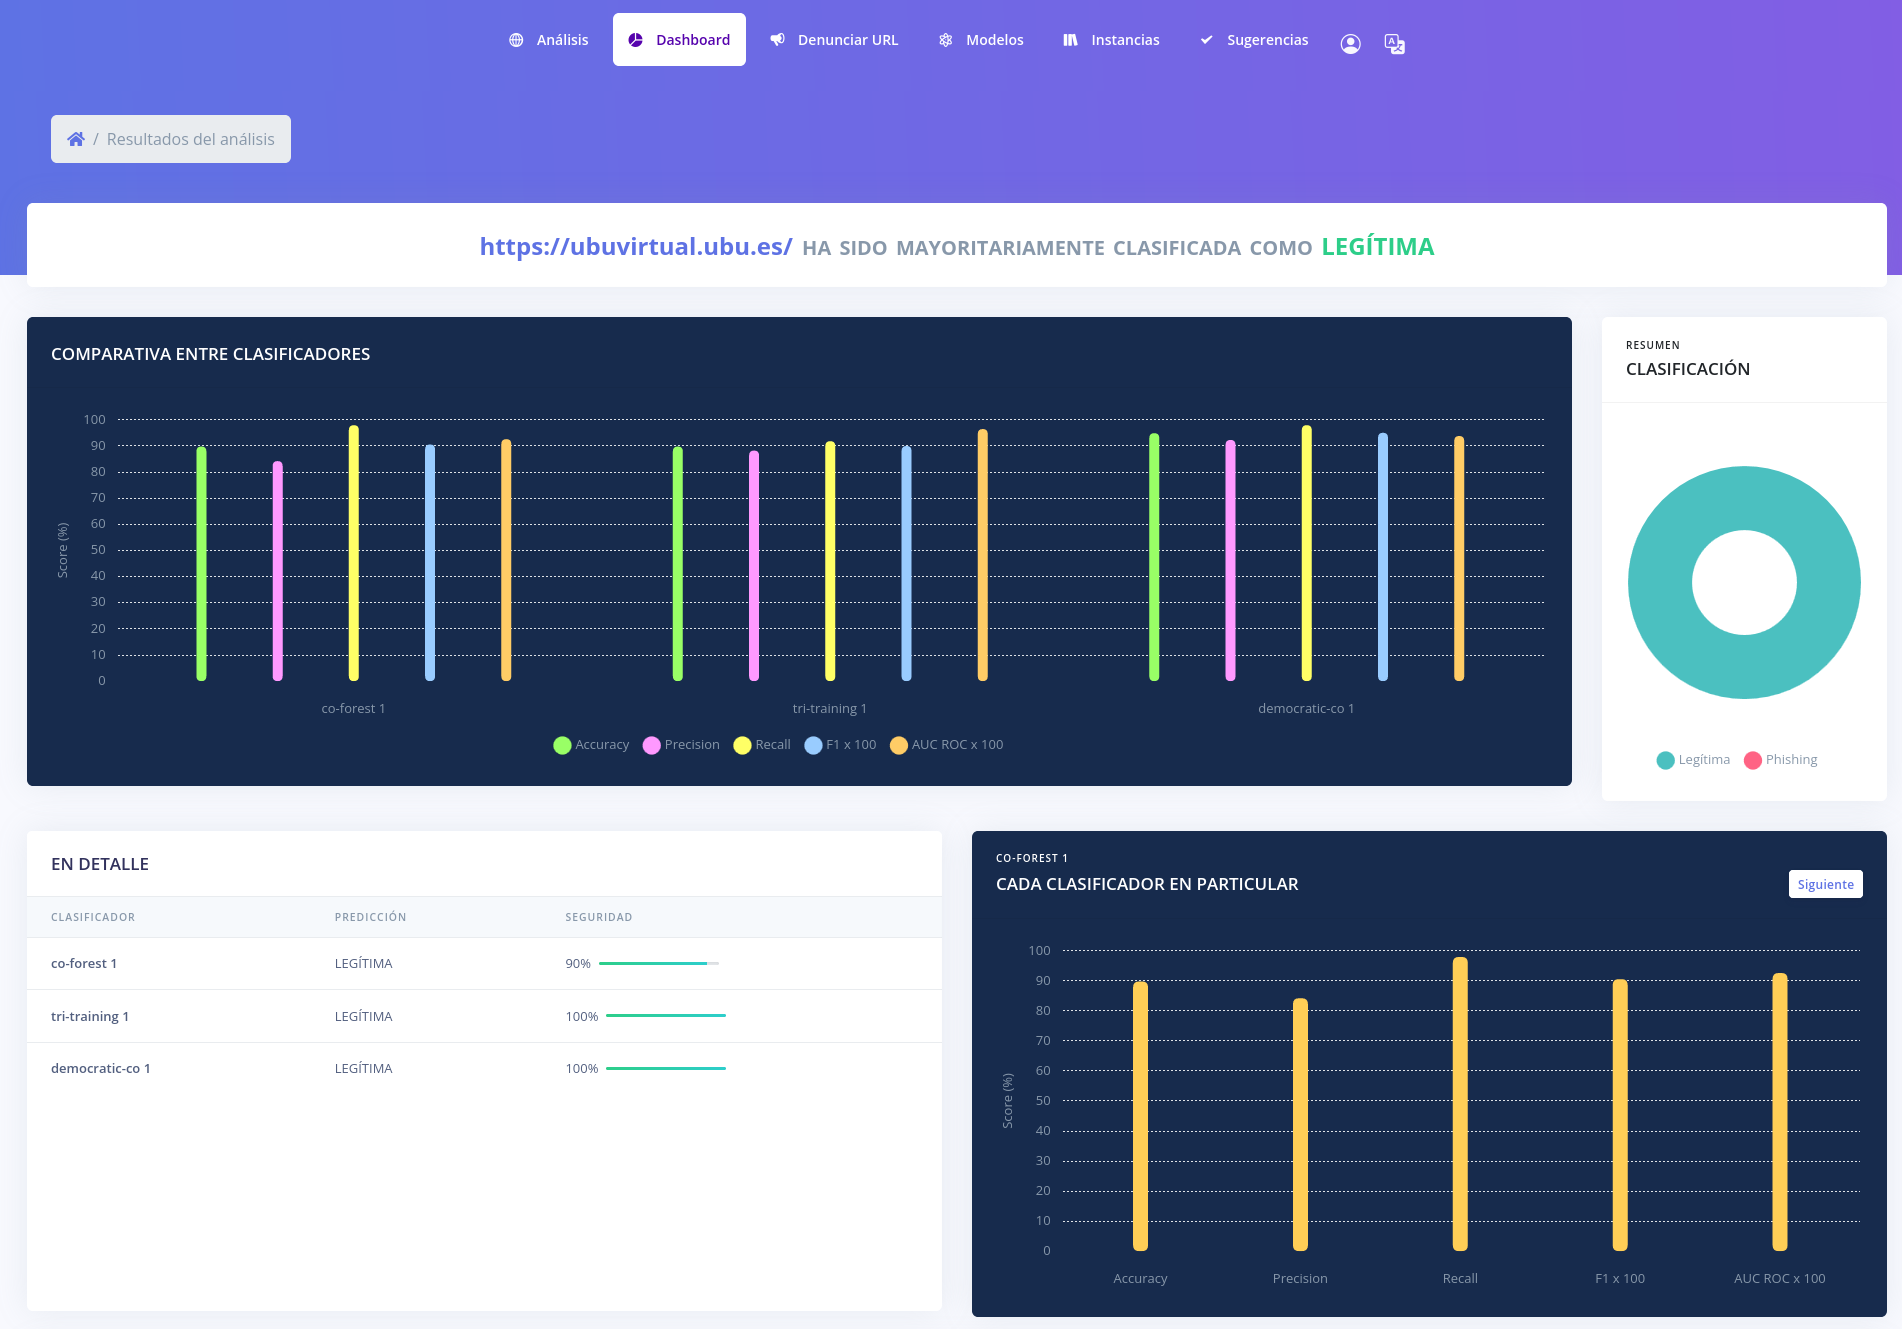
\includegraphics[width=\textwidth]{../img/anexos/user_guide/3_dashboard_1}
	\label{e-3:dashboard-1}
\end{figure}

Si no se ha realizado un análisis rápido, también se mostrará cómo se ha obtenido el vector de características de la URL. Un ejemplo se puede visualizar en la captura~\ref{e-3:dashboard-2}. Pulsando en el icono de la bombilla, se activará un desplegable que muestra información sobre cada característica.

\begin{figure}[h]
	\caption[Manual de usuario: vector de características en el \textit{dashboard}]{Análisis del vector de características mostrado en el dashboard.}
	\centering
	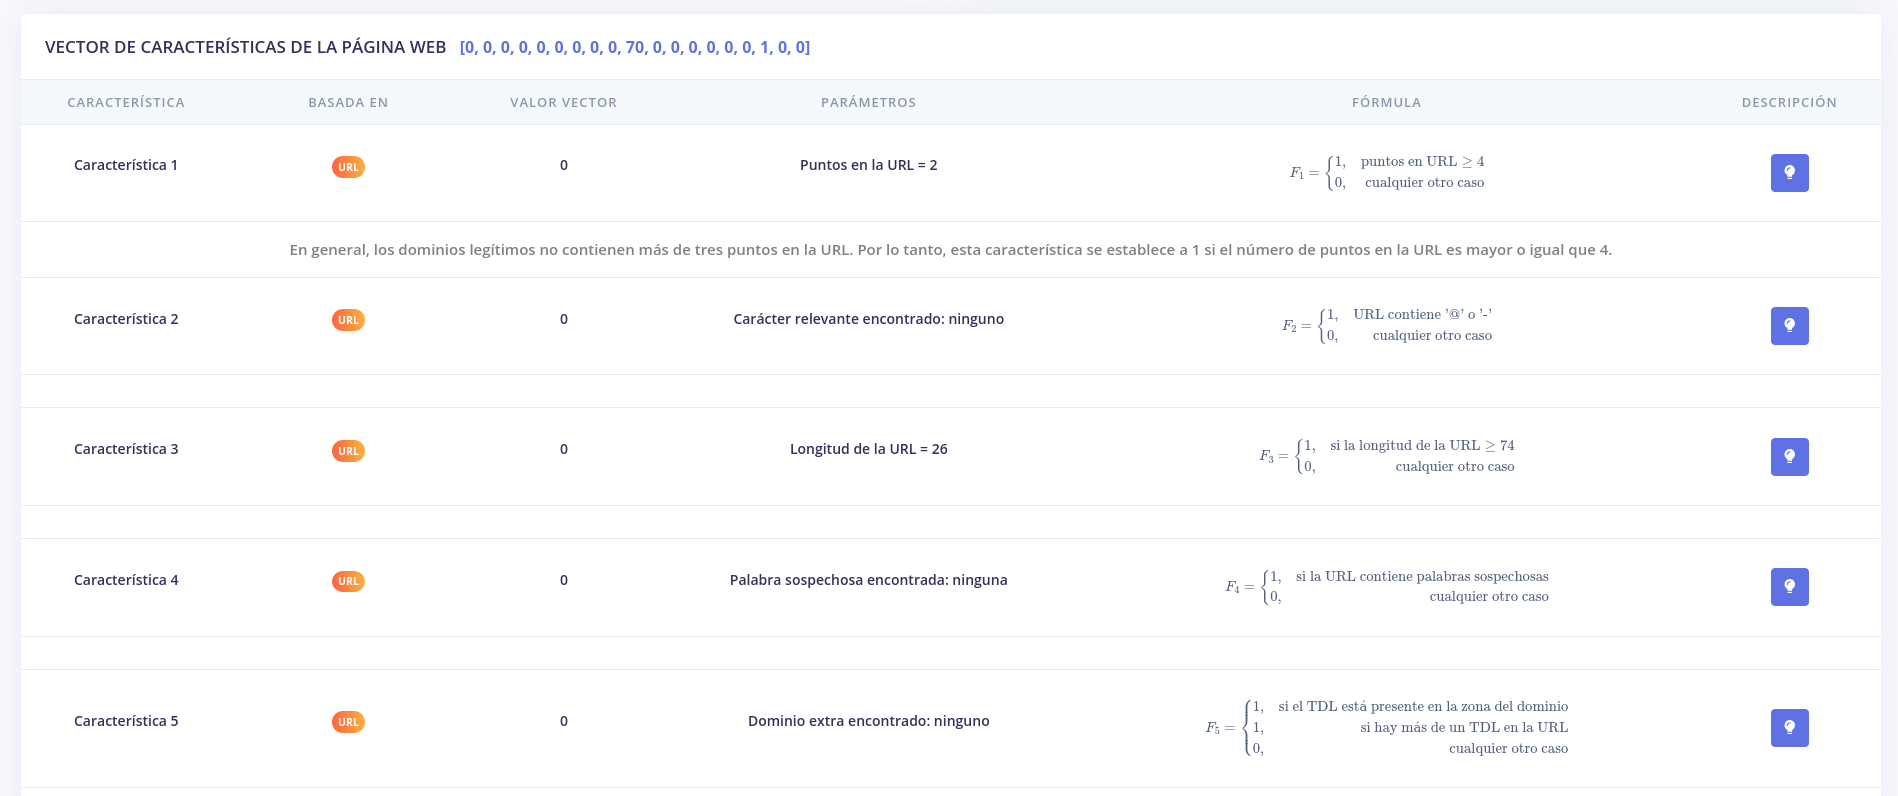
\includegraphics[width=\textwidth]{../img/anexos/user_guide/3_dashboard_2}
	\label{e-3:dashboard-2}
\end{figure}

\begin{figure}[h]
	\caption[Manual de usuario: reportar análisis erróneo]{Reportar análisis realizados erróneamente.}
	\centering
	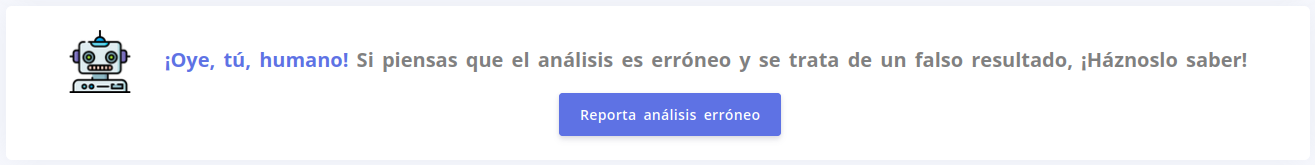
\includegraphics[width=\textwidth]{../img/anexos/user_guide/3_report_false_analysis}
	\label{e-3:report-false-analysis}
\end{figure}

\label{s-e:report-false-analy}
La última funcionalidad del \textit{dashboard} consiste en reportar análisis erróneos. Si se opina que una URL ha sido clasificada incorrectamente, se puede notificar a los administradores pulsando en el botón correspondiente (imagen~\ref{e-3:report-false-analysis}). Luego ellos podrán utilizar esta información para crear nuevos modelos o tomar las medidas que consideren oportunas. La notificación estará disponible en el apartado de <<sugerencias>> (consultar la sección~\ref{s-e:sugerencias} del manual).

\subsection{Denunciar URL}
\label{s-e:report-url}

Si se está seguro de que una URL pertenece a una lista blanca o negra (es decir, se trata de una página legítima o \textit{phishing} confirmada), se puede reportar para que sea revisada por los administradores (consultar la sección~\ref{s-e:sugerencias} del manual) en la página <<denunciar URL>>. Para ello, únicamente habrá que introducir la URL y el tipo de lista a la que pertenece como se muestra en la imagen~\ref{e-3:report-url}.

\begin{figure}[h]
	\caption[Manual de usuario: reportar pertenencia a lista]{Página para reportar pertenencia a lista blanca o lista negra.}
	\centering
	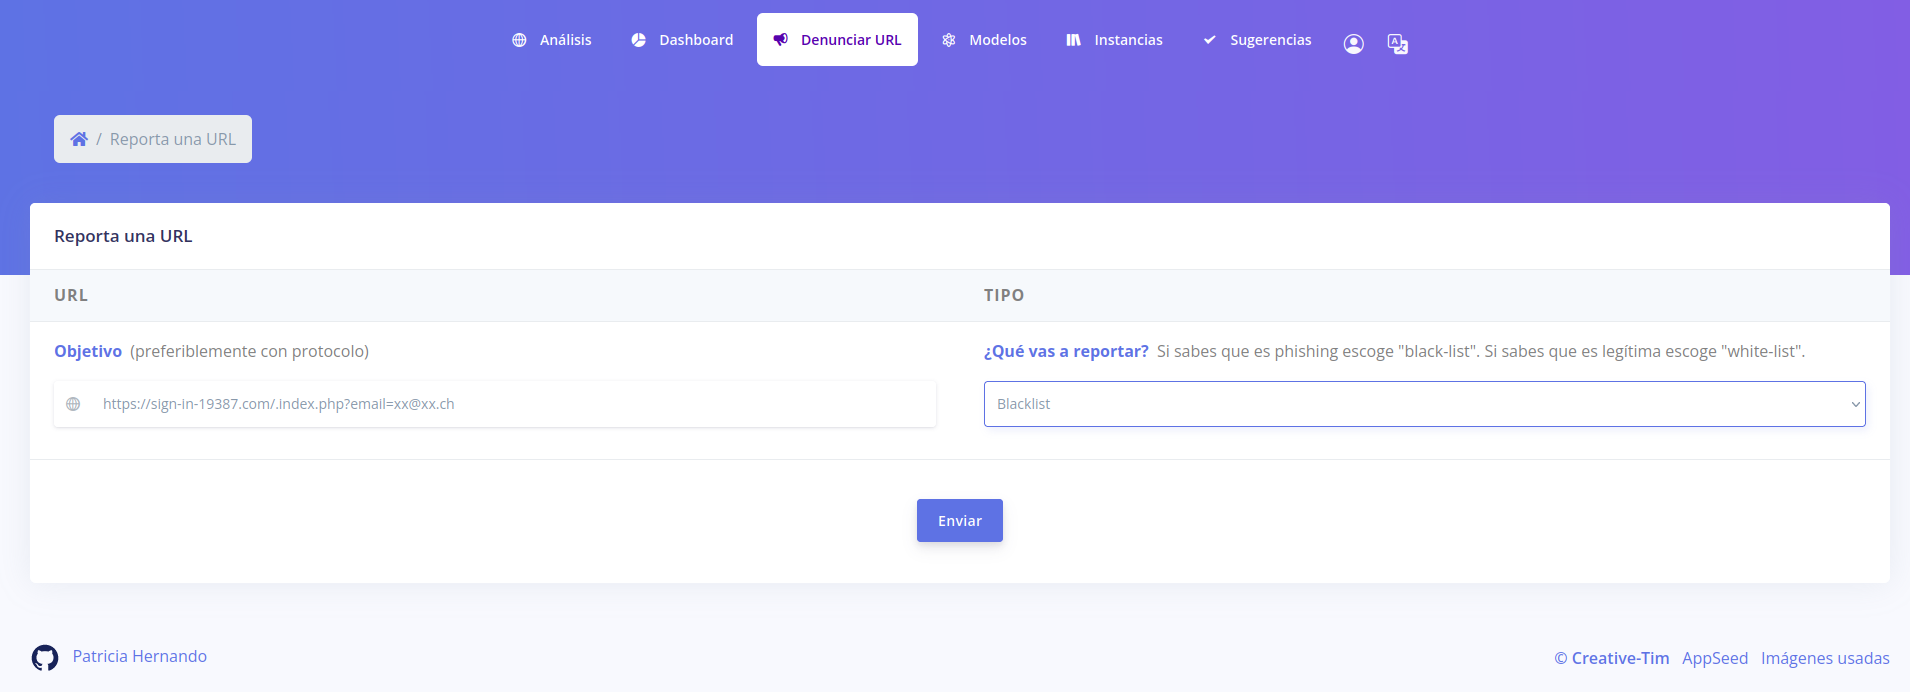
\includegraphics[width=\textwidth]{../img/anexos/user_guide/4_report_url}
	\label{e-3:report-url}
\end{figure}

En caso de que la URL no exista previamente, será incluida en la sección de <<instancias>> (consultar sección~\ref{s-e:instances} del manual), aunque no se generará su vector de características para evitar que el usuario tenga que esperar. Posteriormente los administradores podrán ejecutar esta tarea. Es destacable que las URL sin vector de características no podrán ser utilizadas para realizar análisis rápidos ni entrenar o evaluar modelos.


\subsection{Modelos}
\label{s-e:models}

\begin{figure}[h]
	\caption[Manual de usuario: página de modelos]{Página de administración de modelos.}
	\centering
	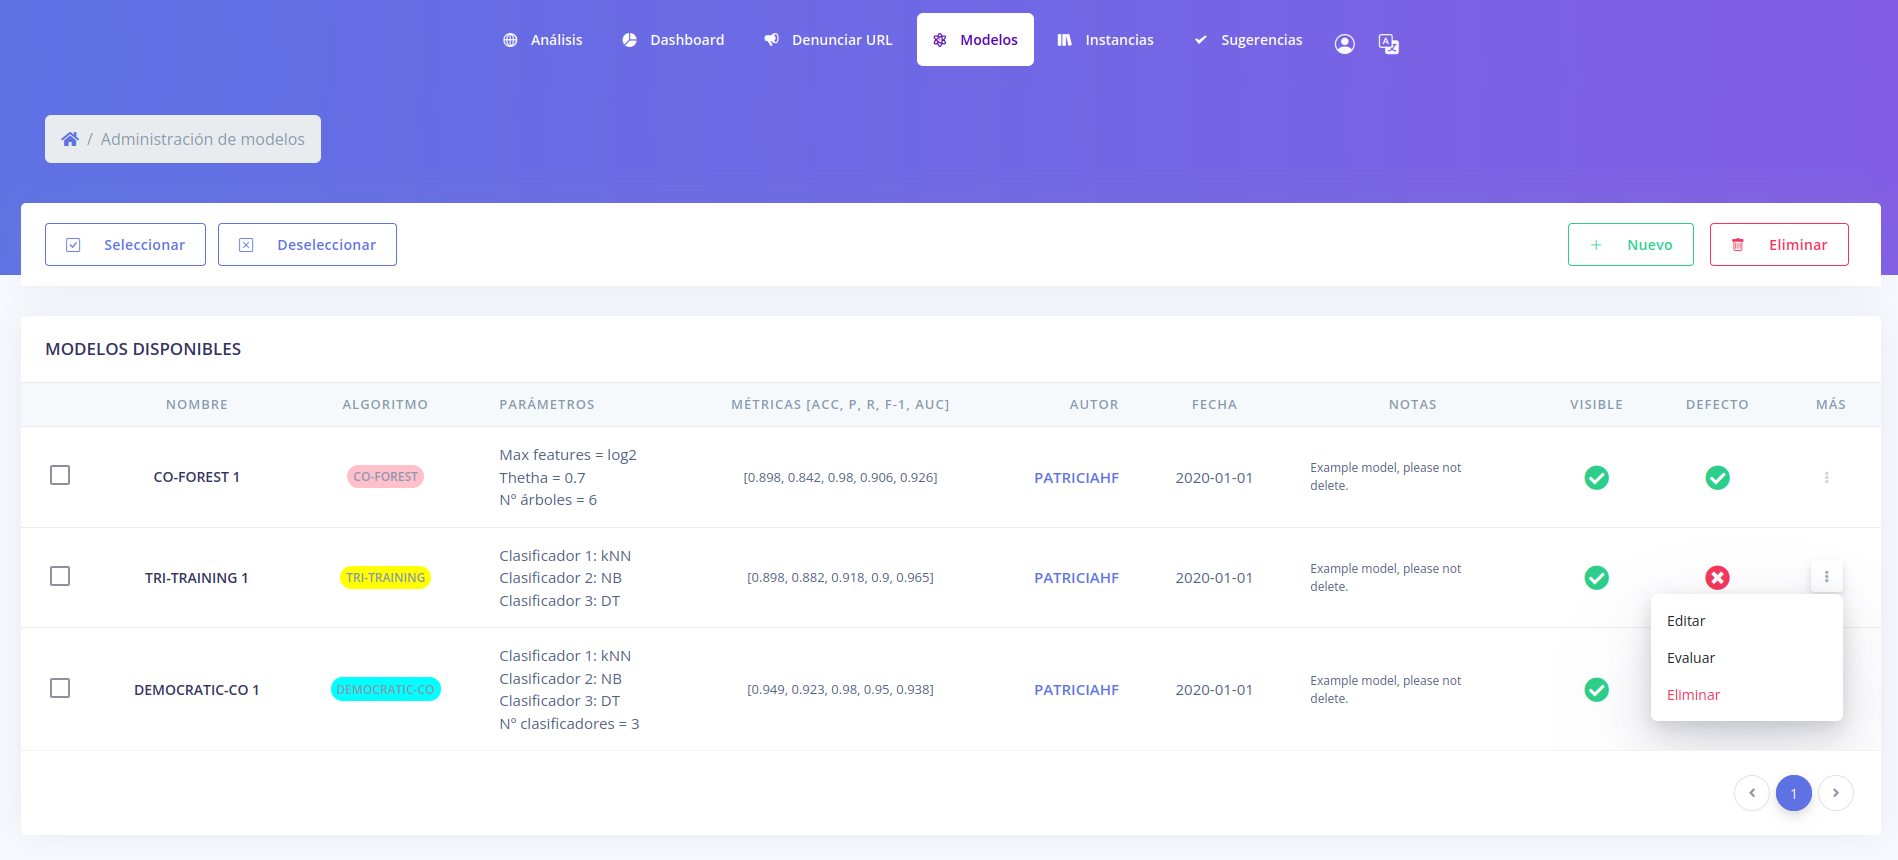
\includegraphics[width=\textwidth]{../img/anexos/user_guide/5_models}
	\label{e-5:models}
\end{figure}

\begin{figure}[h]
	\caption[Manual de usuario: nuevo modelo]{Formulario de creación de nuevos modelos.}
	\centering
	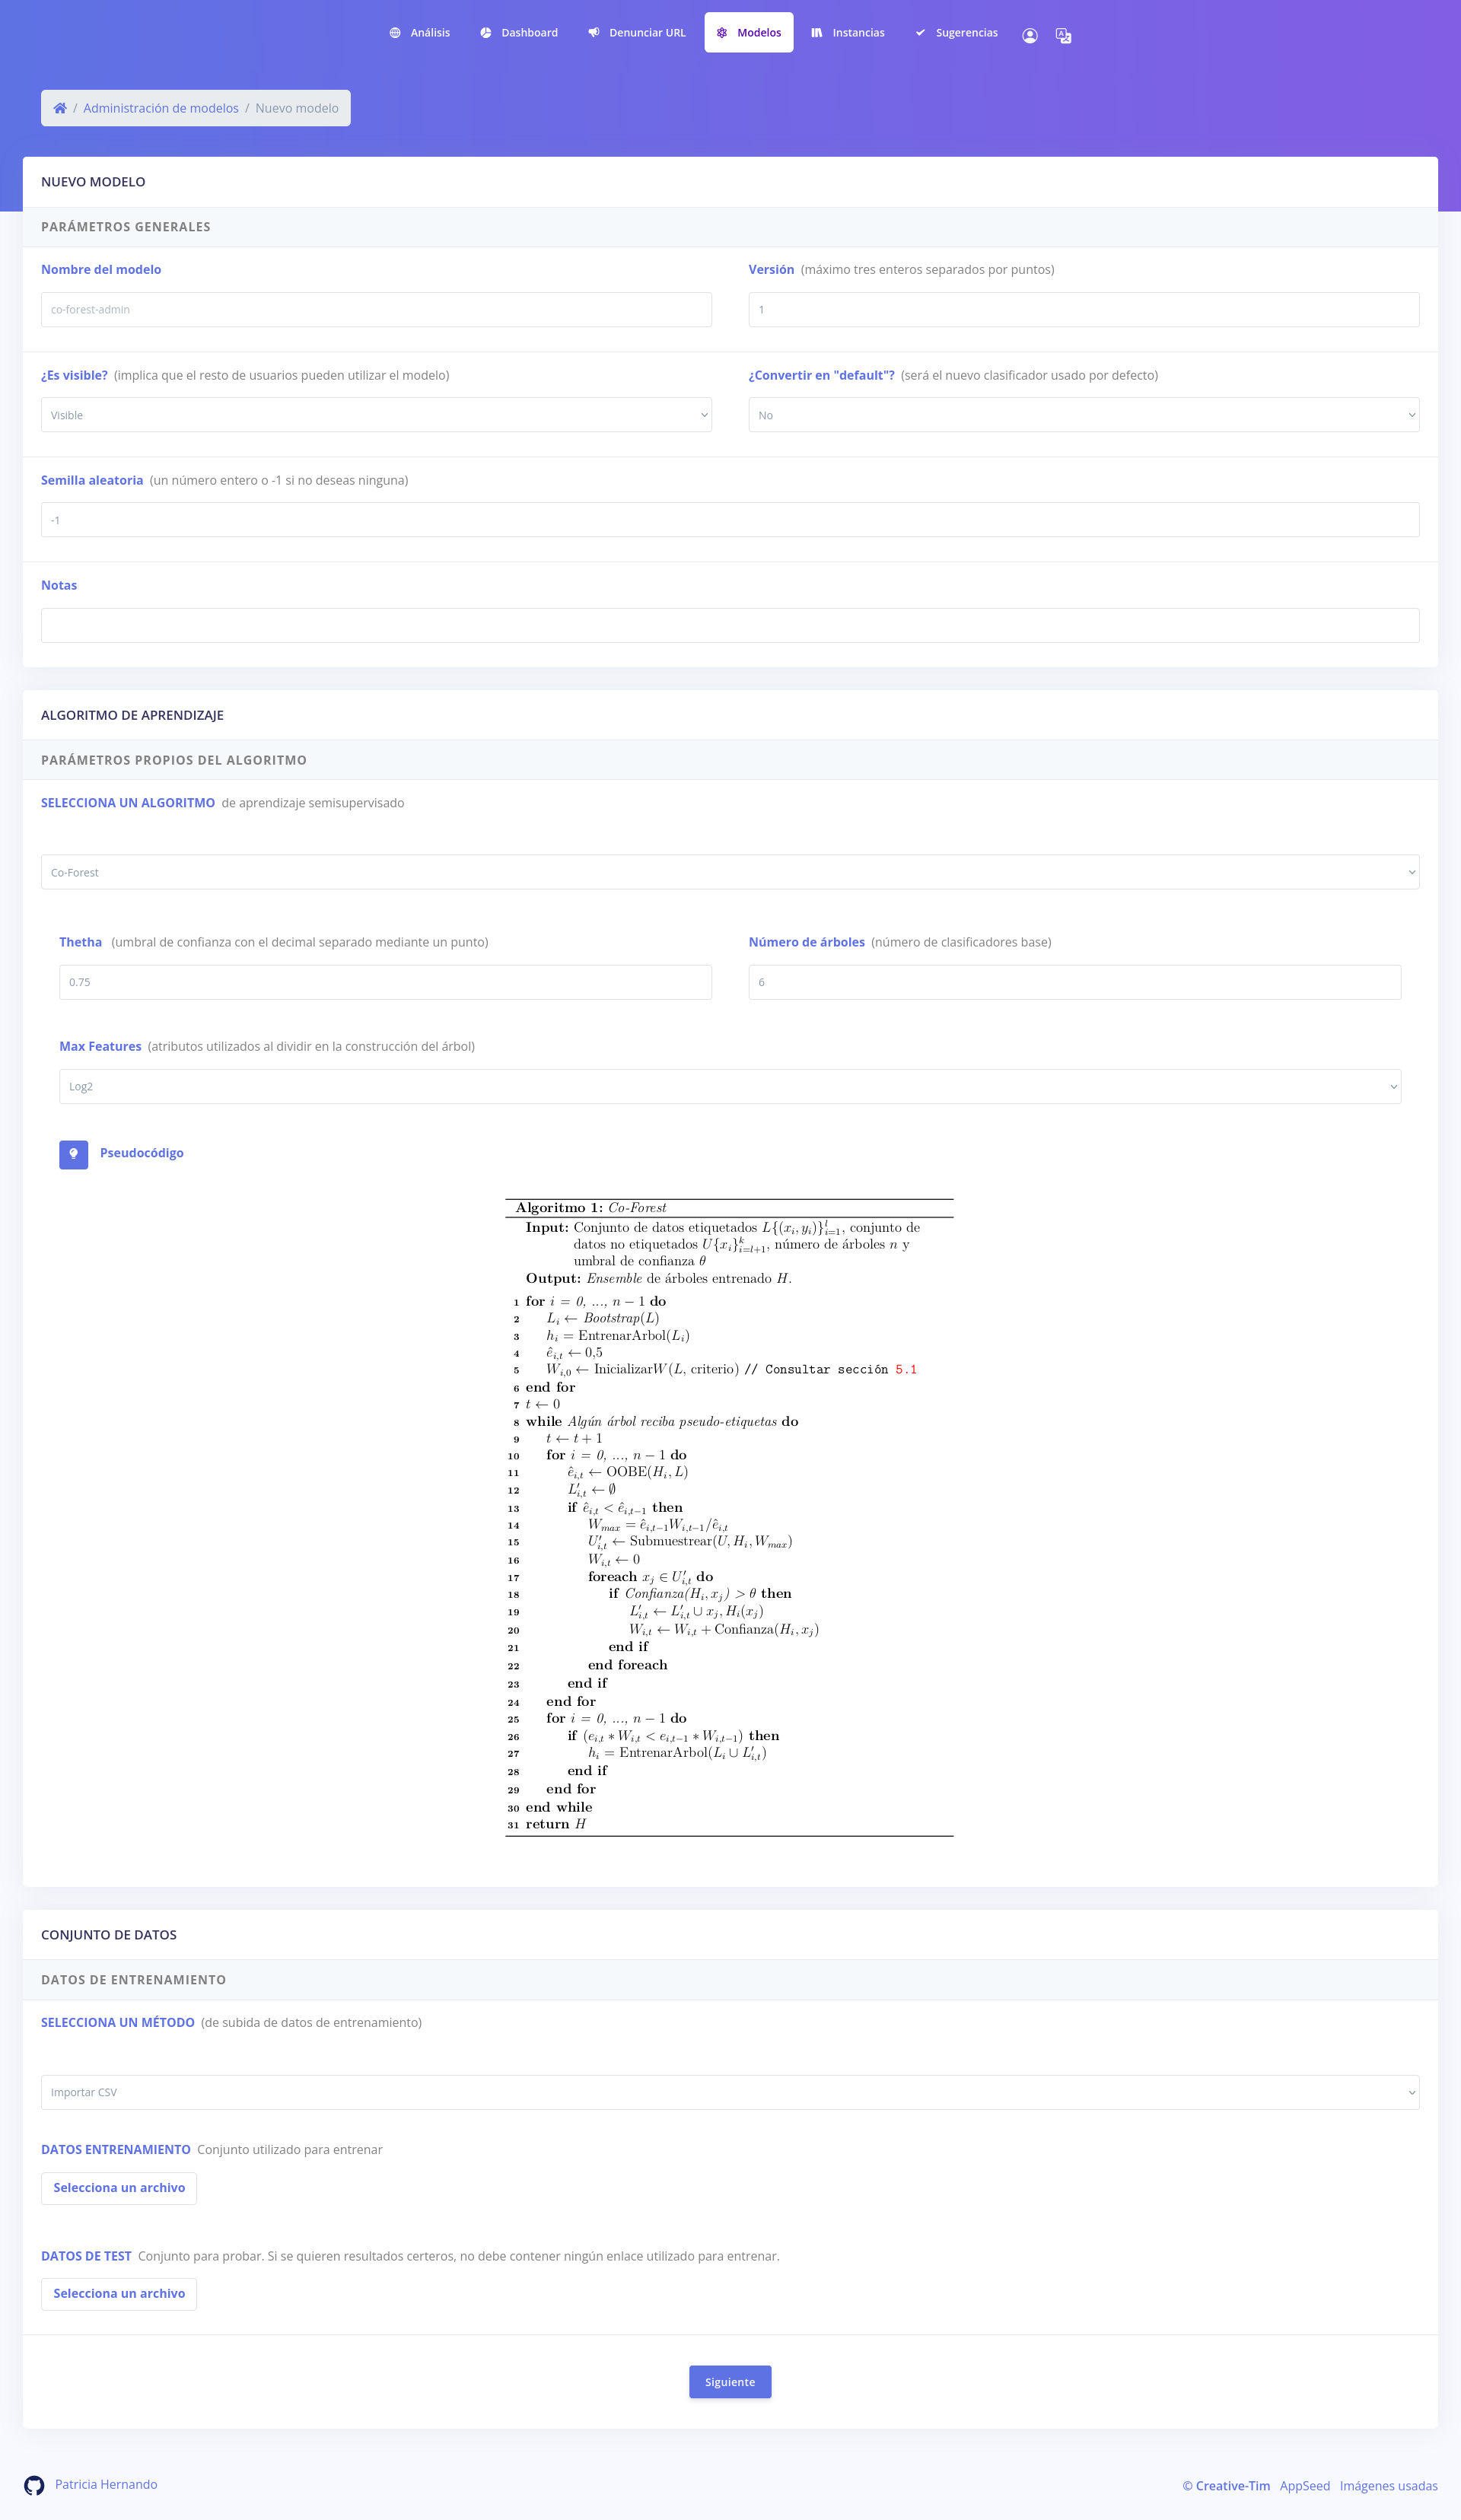
\includegraphics[width=\textwidth]{../img/anexos/user_guide/5_new_model}
	\label{e-5:new-model}
\end{figure}

\begin{figure}[h]
	\caption[Manual de usuario: editar modelo]{Formulario de edición de modelos existentes.}
	\centering
	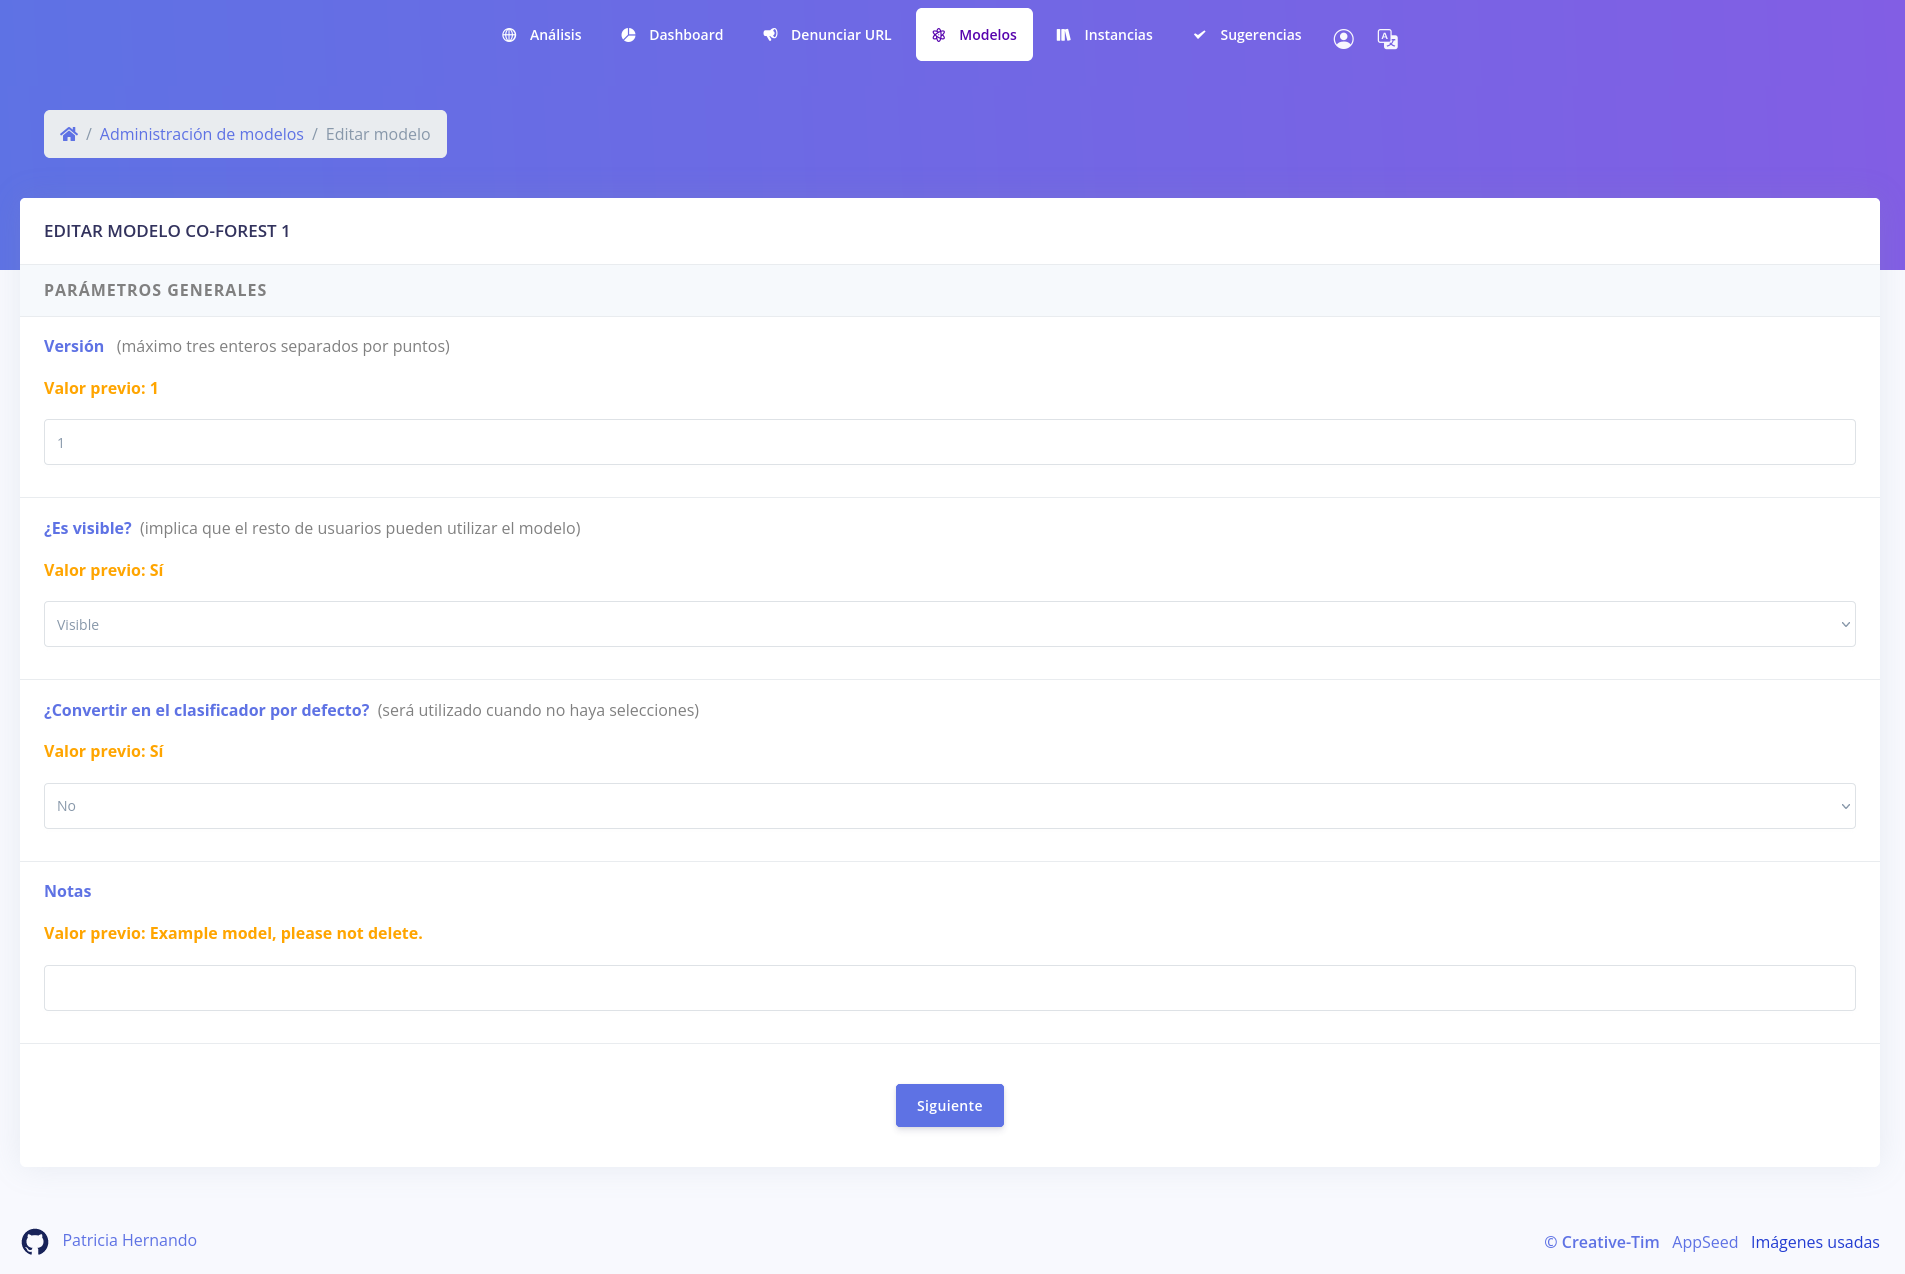
\includegraphics[width=\textwidth]{../img/anexos/user_guide/5_edit_model}
	\label{e-5:edit-model}
\end{figure}

\begin{figure}[h]
	\caption[Manual de usuario: evaluar modelo]{Página de evaluación de modelos existentes.}
	\centering
	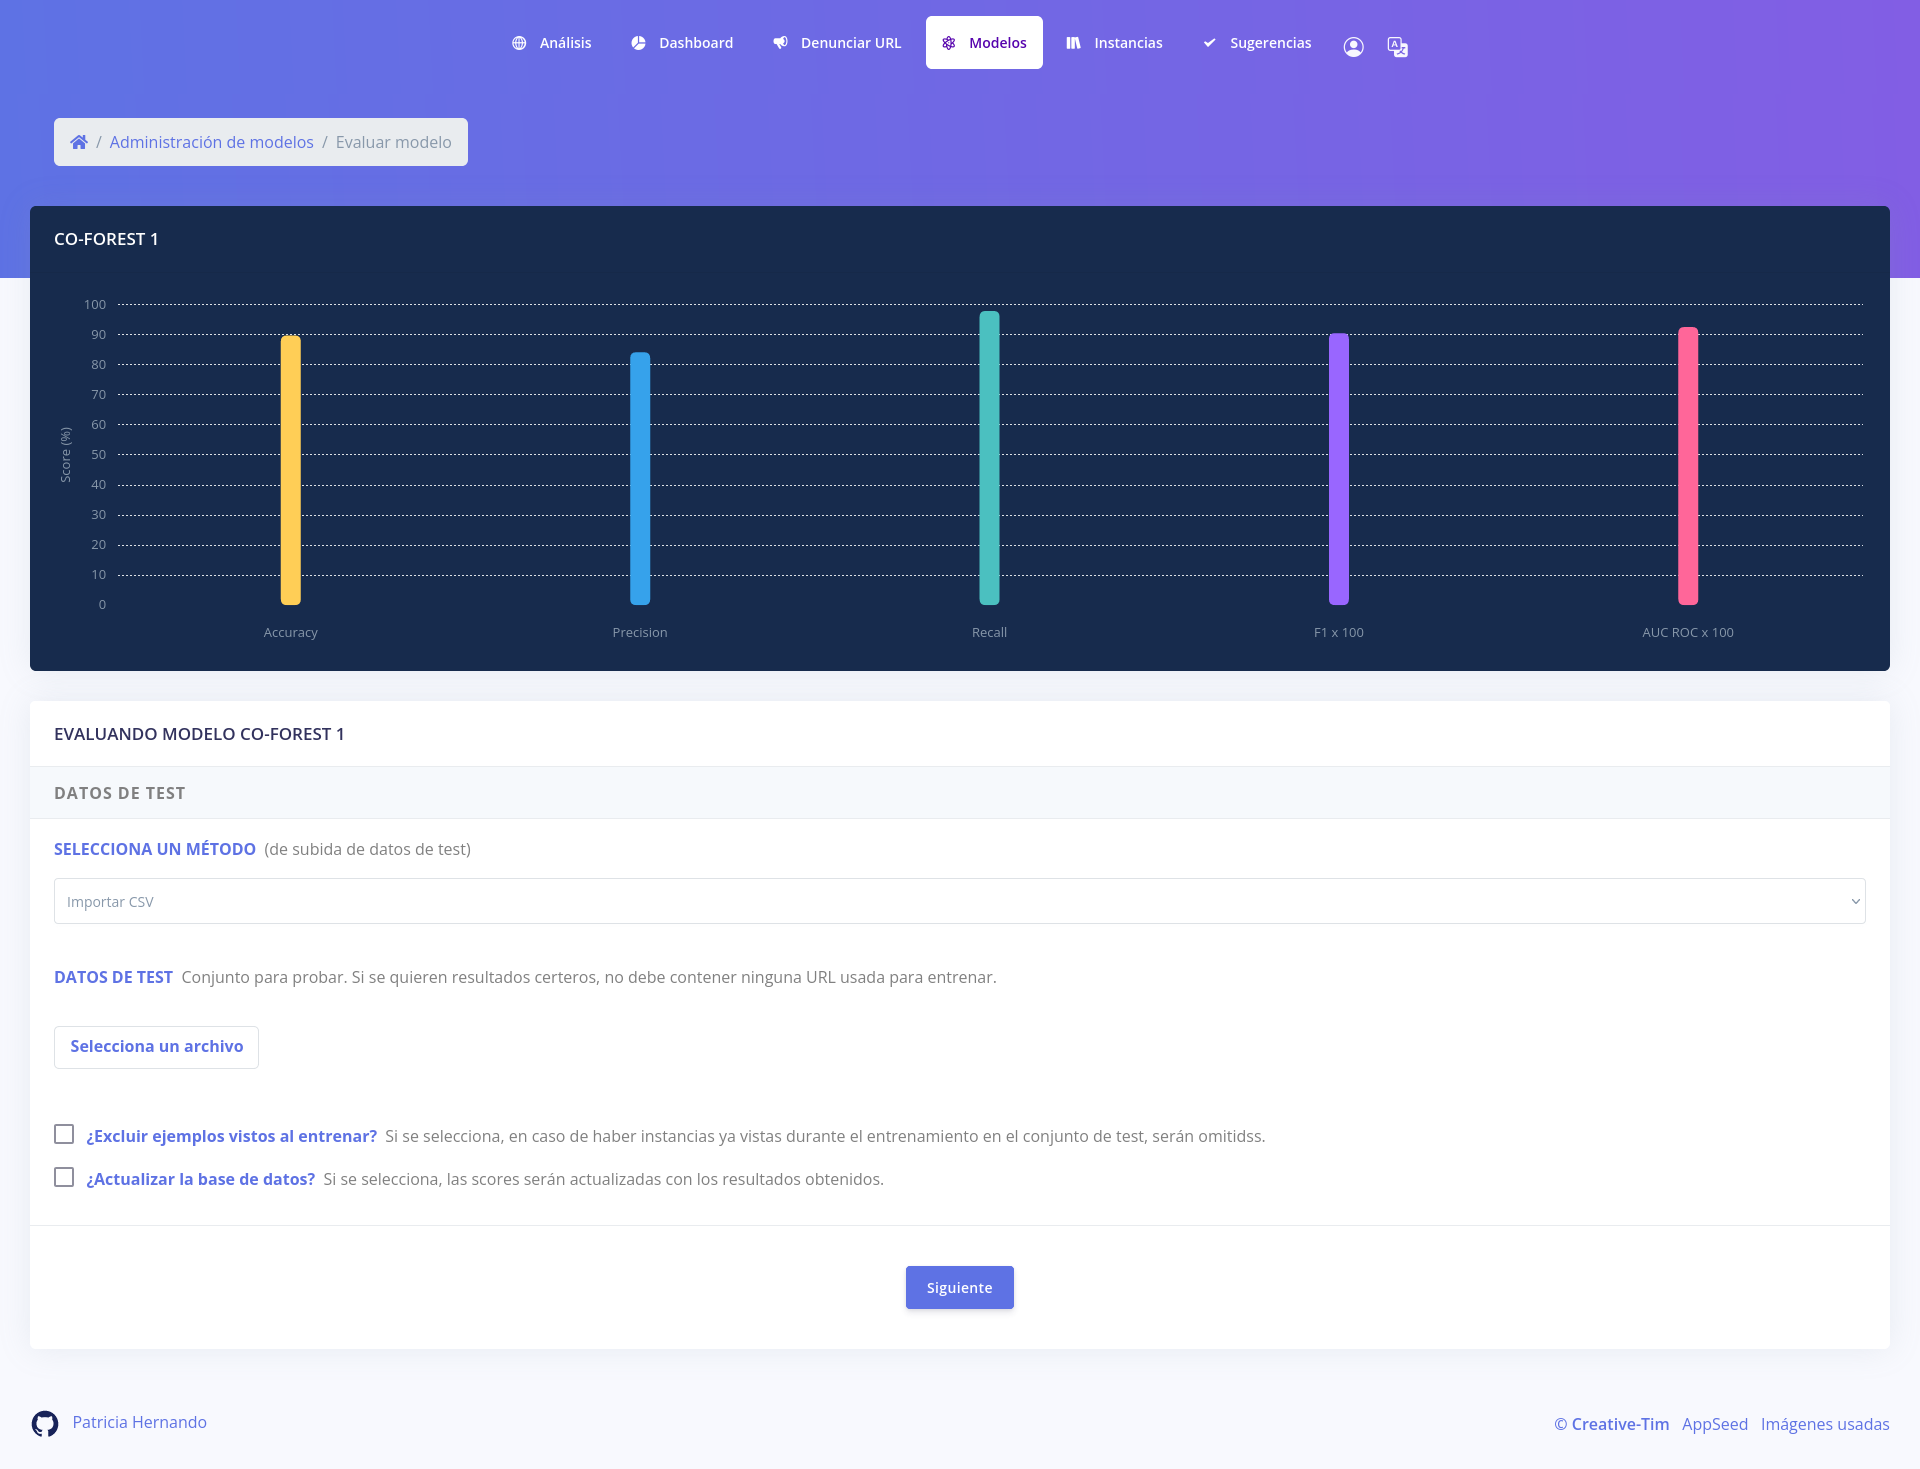
\includegraphics[width=\textwidth]{../img/anexos/user_guide/5_test_model}
	\label{e-5:test-model}
\end{figure}


\subsection{Instancias}
\label{s-e:instances}

\begin{figure}[h]
	\caption[Manual de usuario: página de instancias]{Página de administración de instancias.}
	\centering
	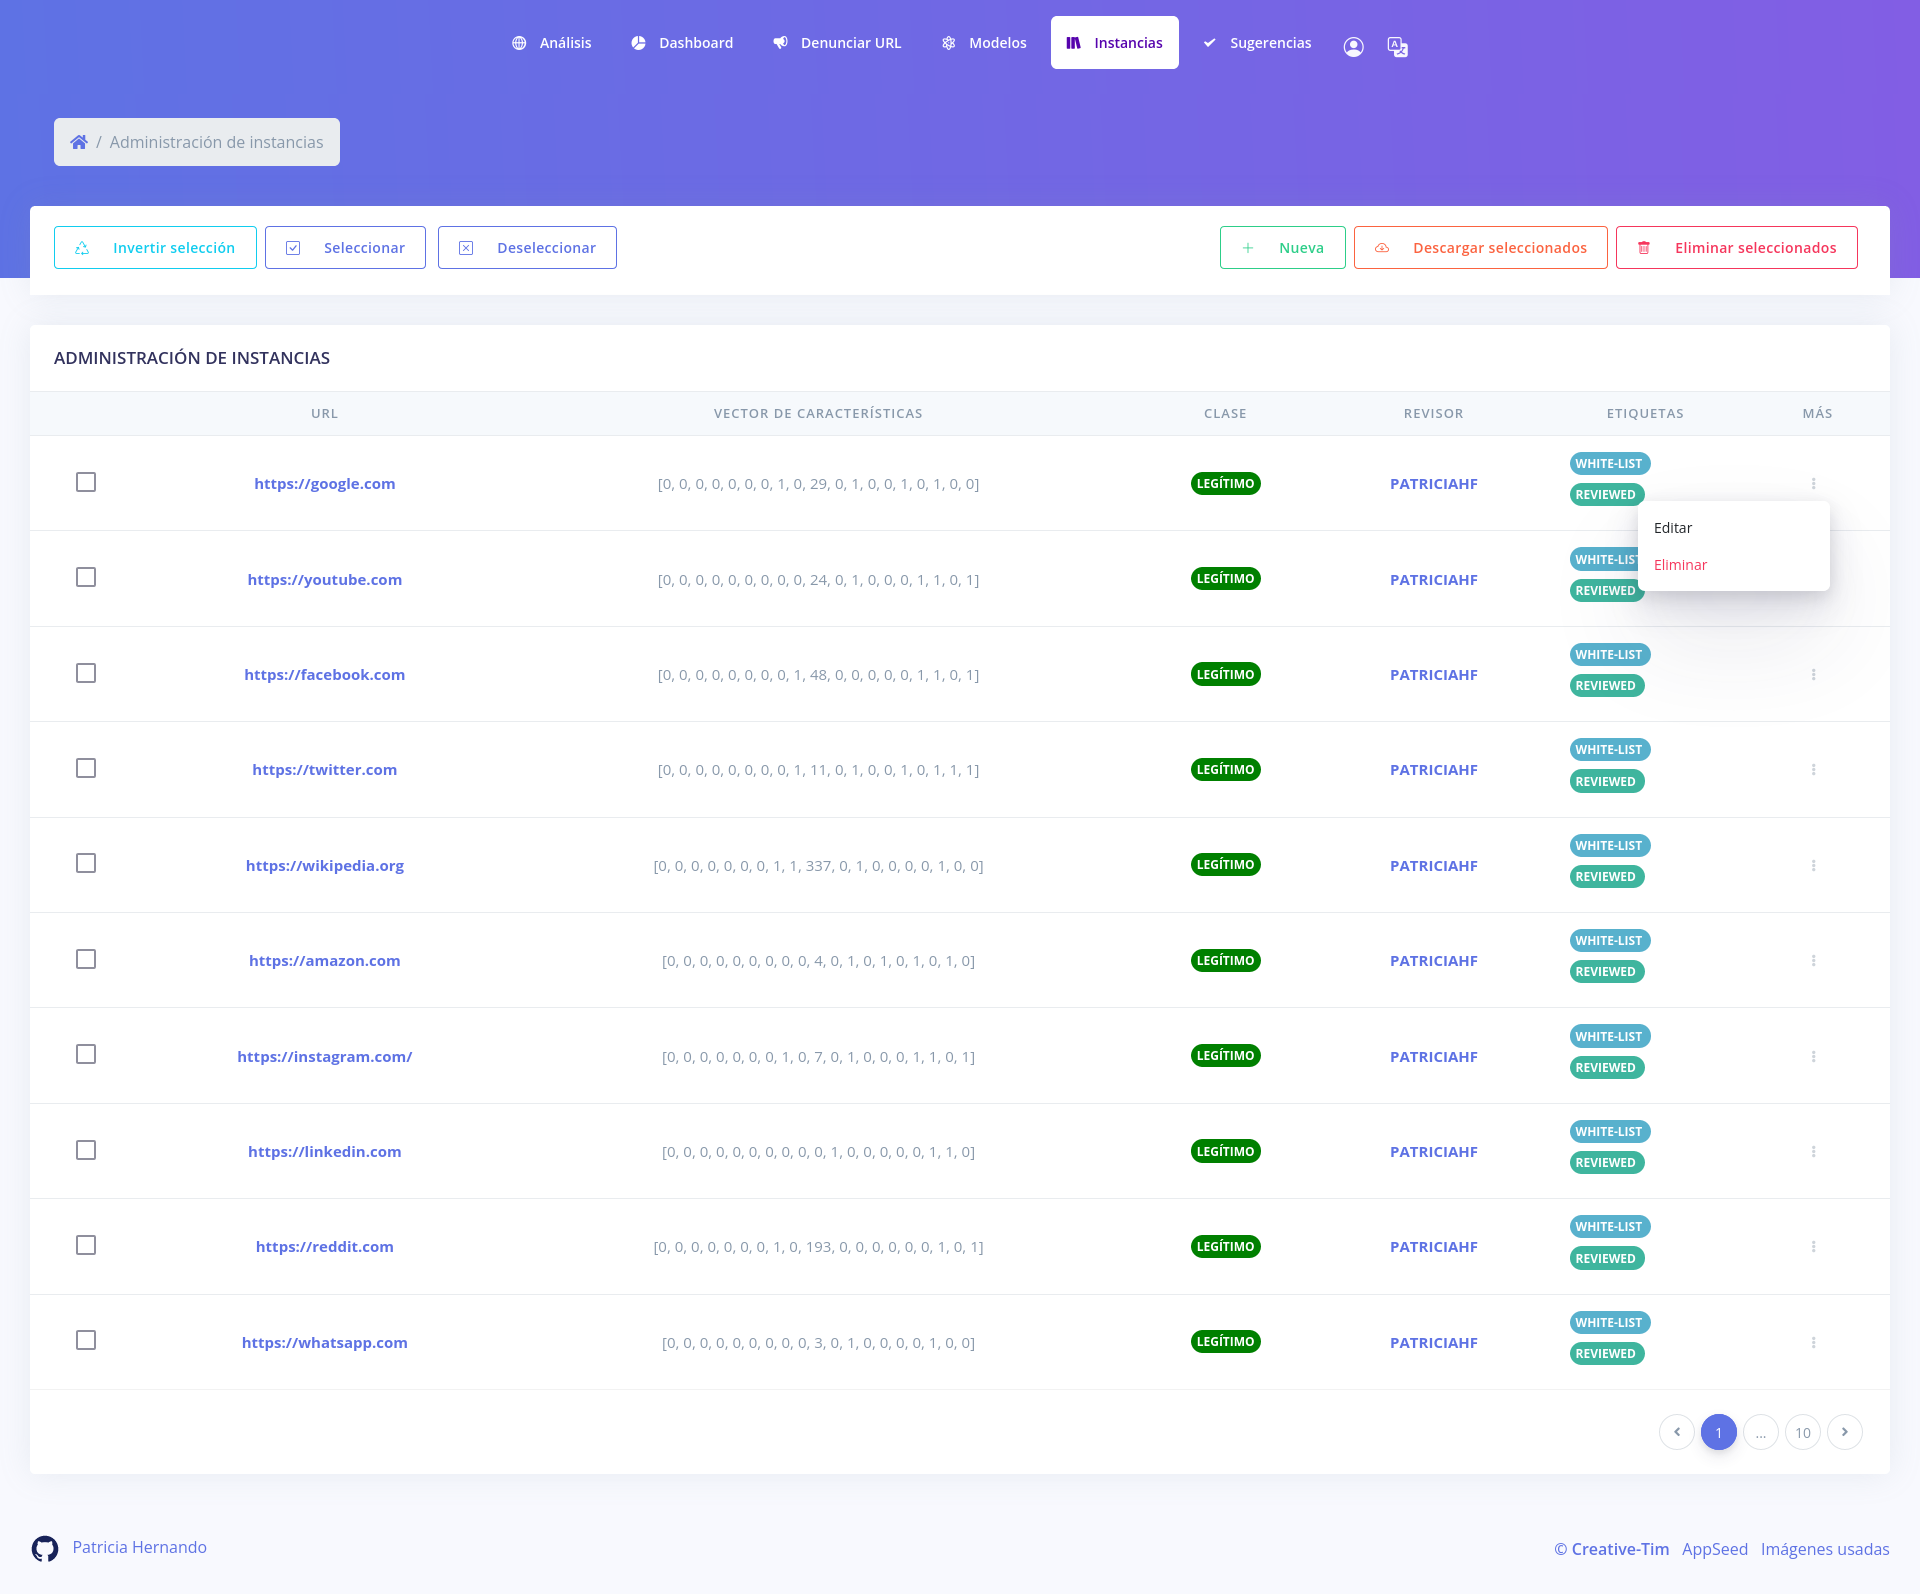
\includegraphics[width=\textwidth]{../img/anexos/user_guide/6_instances}
	\label{e-5:instances}
\end{figure}

\begin{figure}[h]
	\caption[Manual de usuario: nueva instancia]{Formulario de creación de nuevas instancias.}
	\centering
	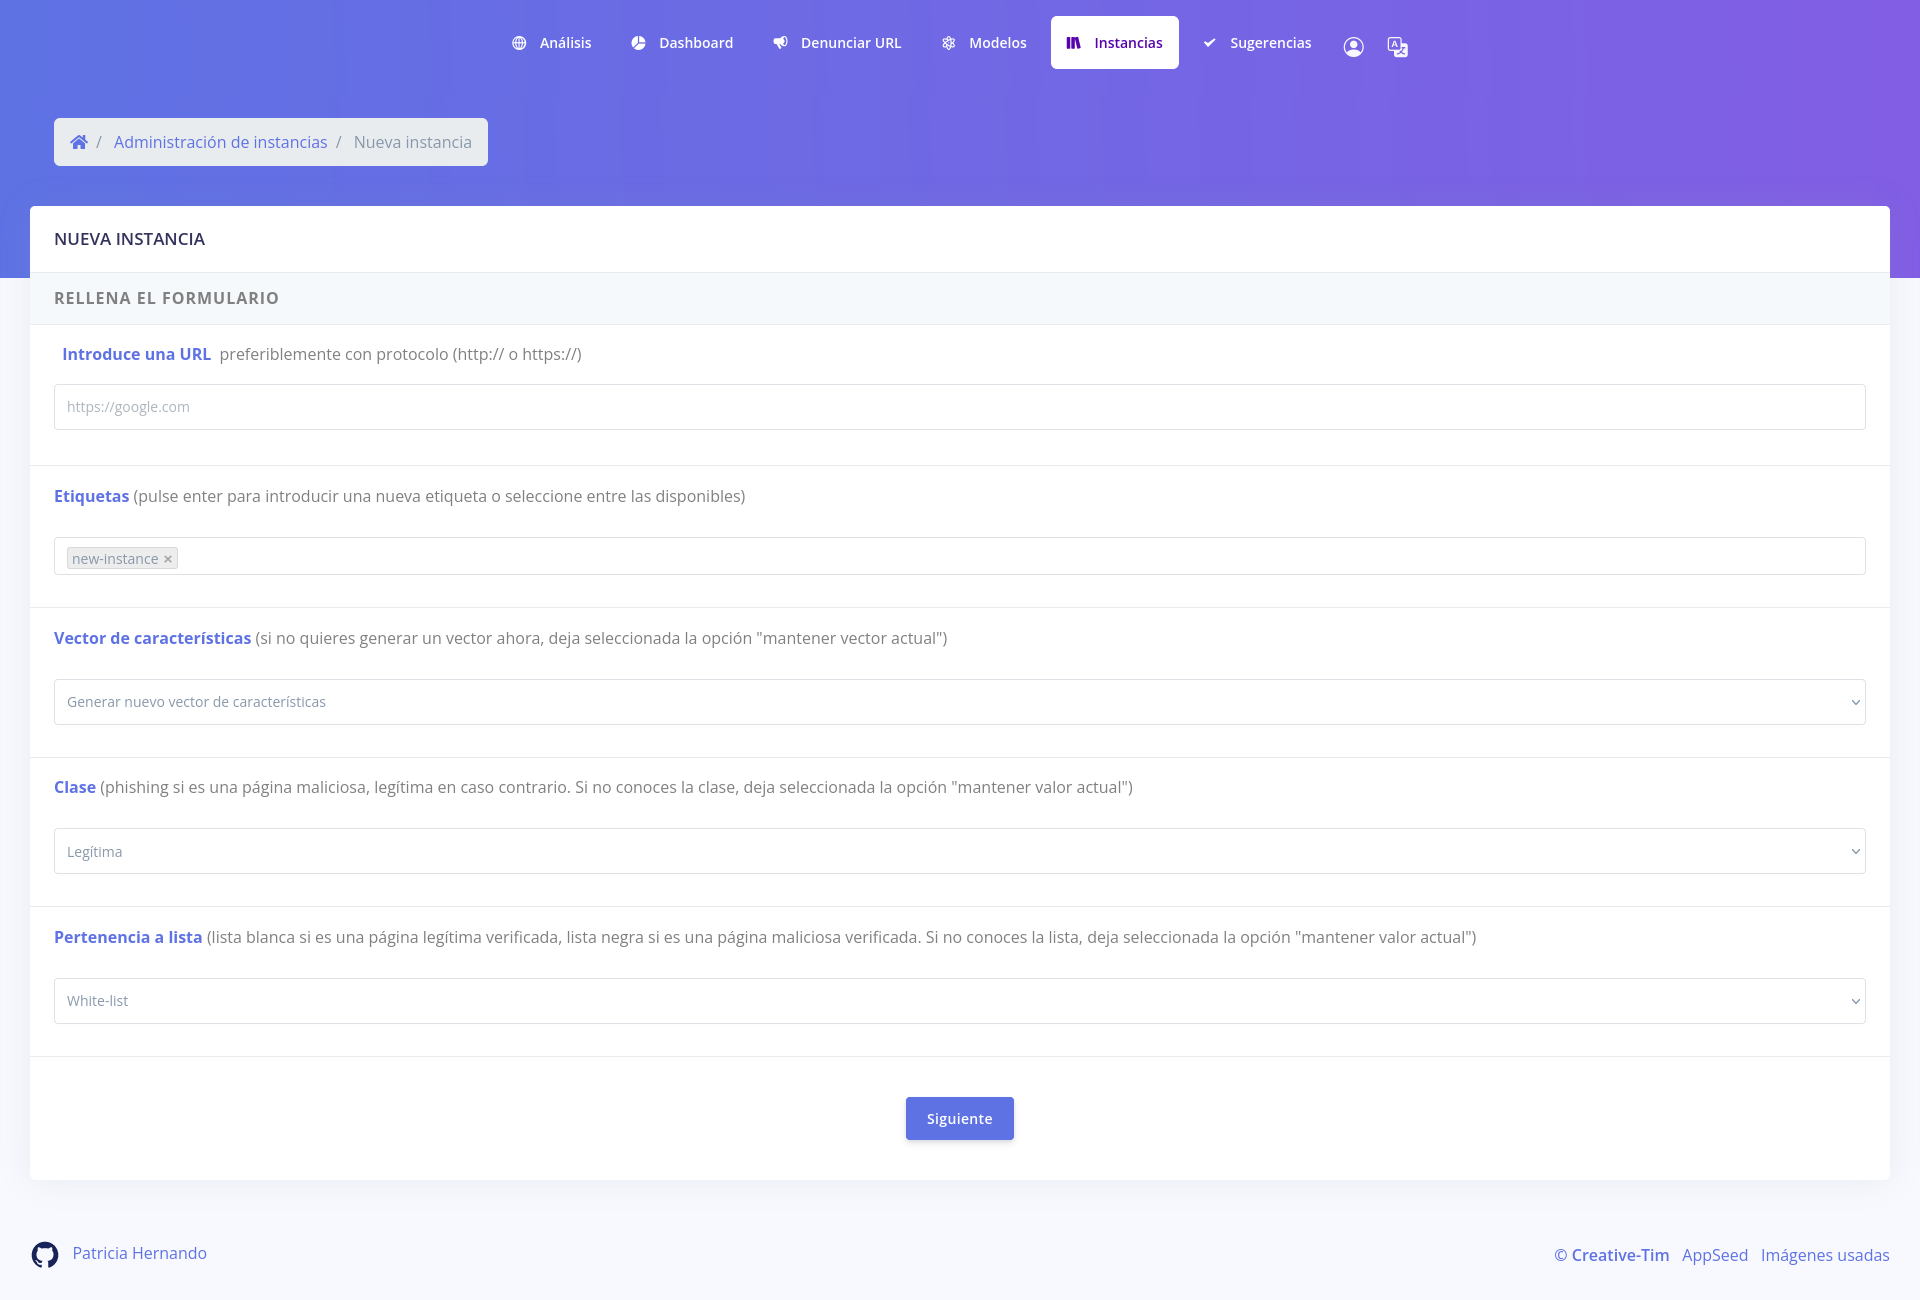
\includegraphics[width=\textwidth]{../img/anexos/user_guide/6_new_instance}
	\label{e-5:new-instance}
\end{figure}

\begin{figure}[h]
	\caption[Manual de usuario: editar instancia]{Formulario de edición de instancias existentes.}
	\centering
	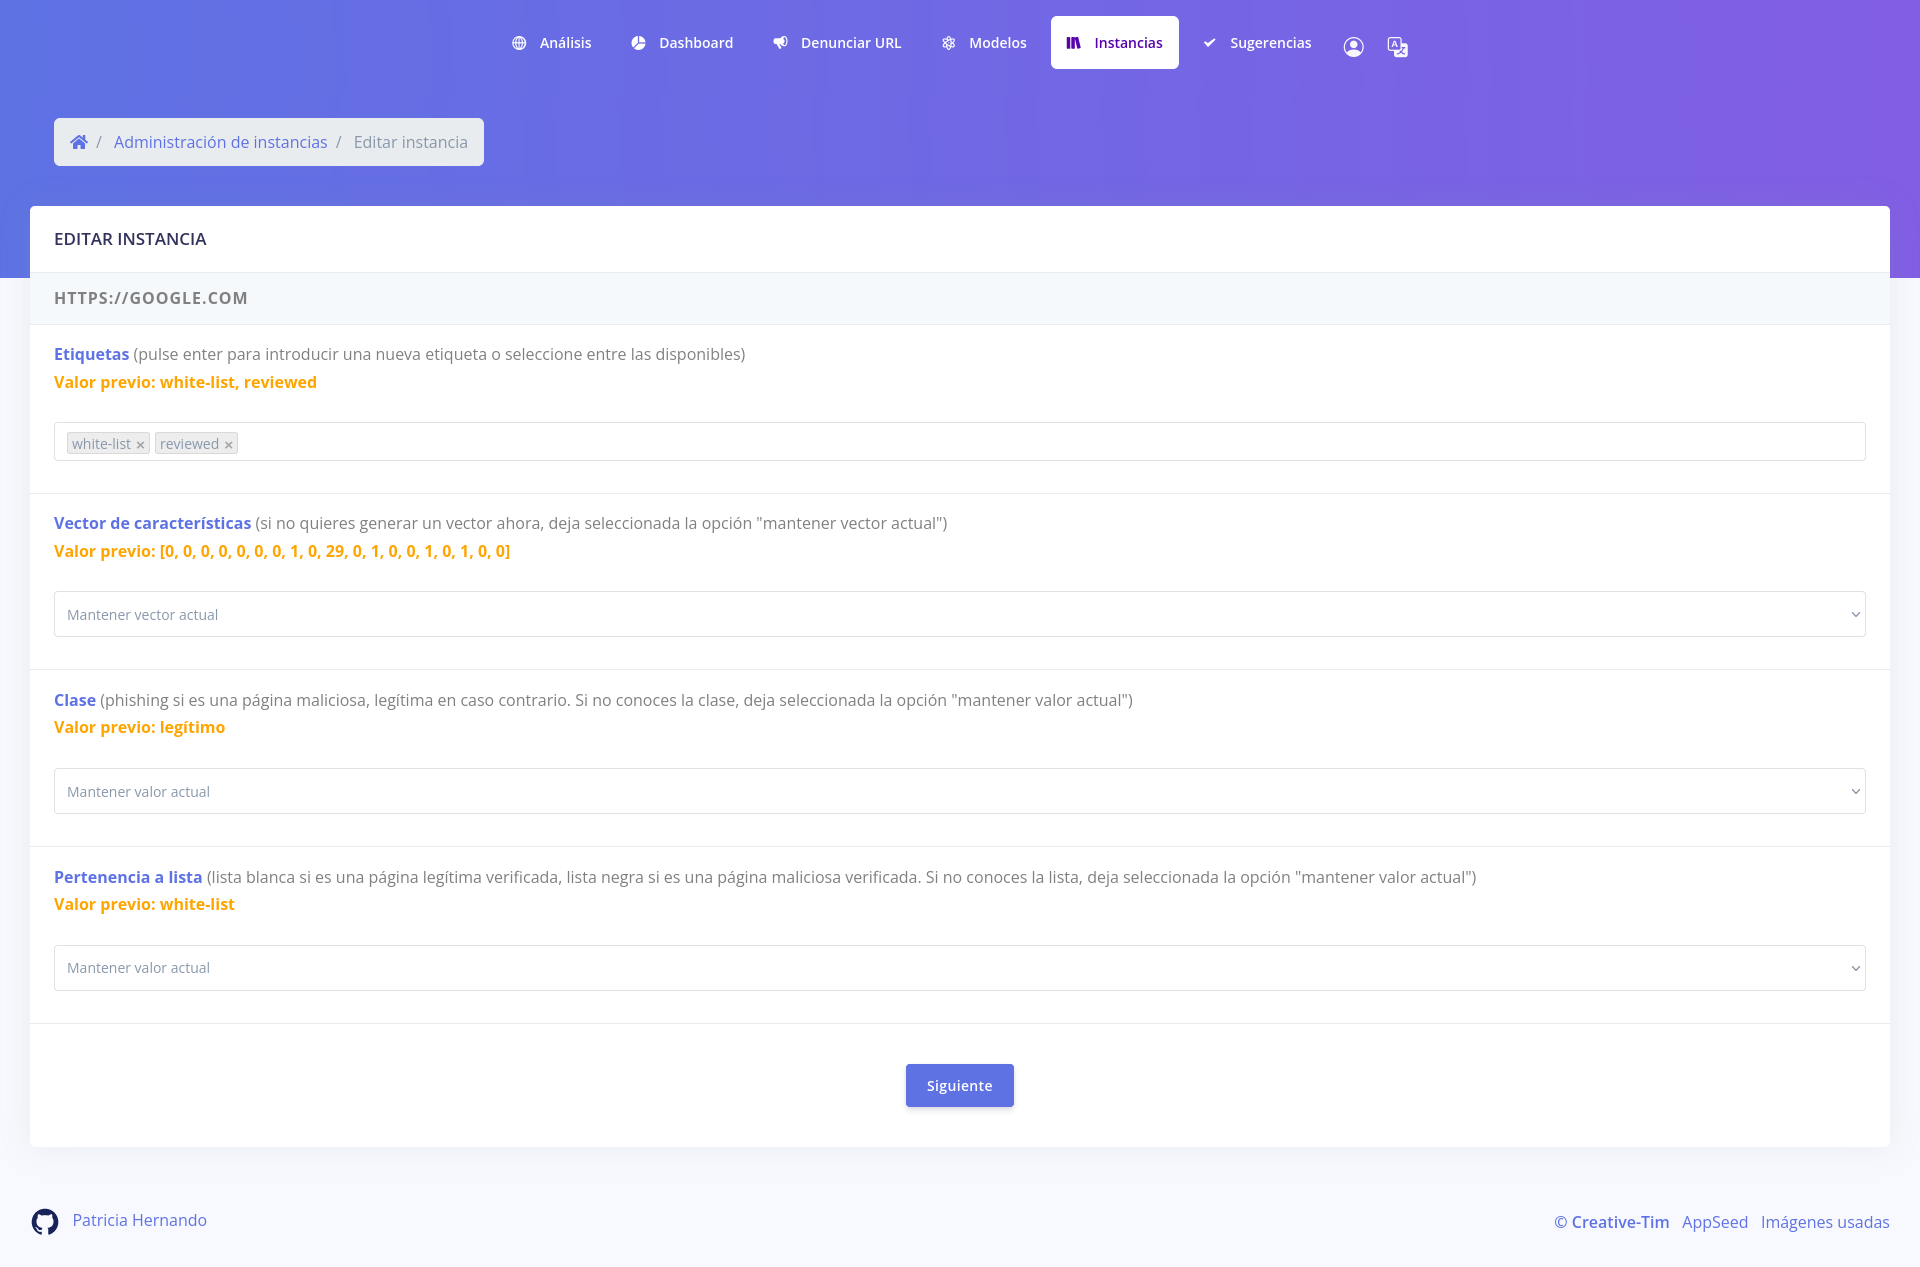
\includegraphics[width=\textwidth]{../img/anexos/user_guide/6_edit_instance}
	\label{e-5:edit-instance}
\end{figure}

\begin{figure}[h]
	\caption[Manual de usuario: etiquetas predeterminadas]{Menú con las etiquetas predeterminadas.}
	\centering
	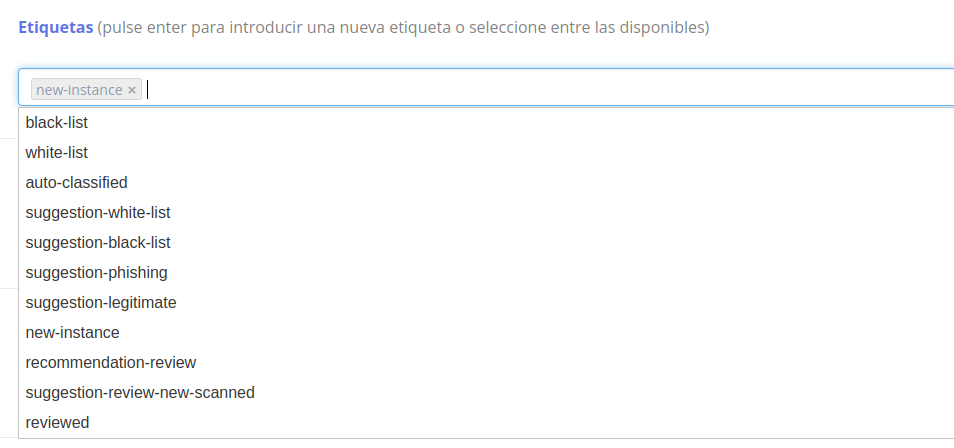
\includegraphics[width=\textwidth]{../img/anexos/user_guide/6_labels}
	\label{e-6:labels}
\end{figure}

\begin{figure}[h]
	\caption[Manual de usuario: ejemplos de etiquetas]{Instancias con variedad de etiquetas.}
	\centering
	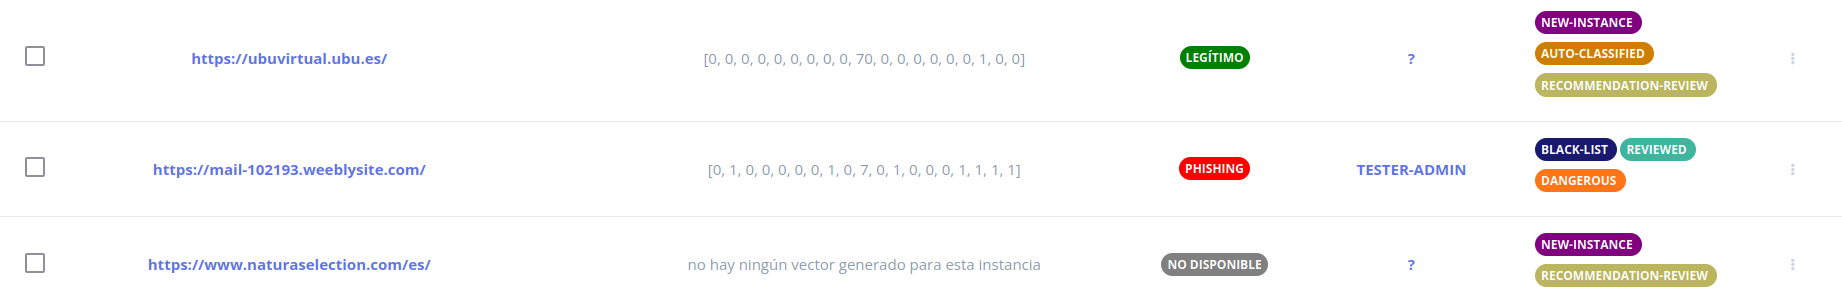
\includegraphics[width=\textwidth]{../img/anexos/user_guide/6_instances_more_labels}
	\label{e-6:more-labels}
\end{figure}

\subsection{Sugerencias}
\label{s-e:sugerencias}

Cuando un usuario registrado reporta un análisis que considera erróneo (consultar sección~\ref{s-e:report-false-analy}) o denuncia una URL por pertenecer a una lista blanca o negra (consultar sección~\ref{s-e:report-url}), se crea una nueva entrada en la sección de <<sugerencias>>. También se crean nuevas sugerencias cuando un usuario registrado analiza una URL (para recordar al administrador que revise la nueva instancia).

\begin{figure}[h]
	\caption[Manual de usuario: administrar sugerencias]{Página de administración de sugerencias o \textit{reports}.}
	\centering
	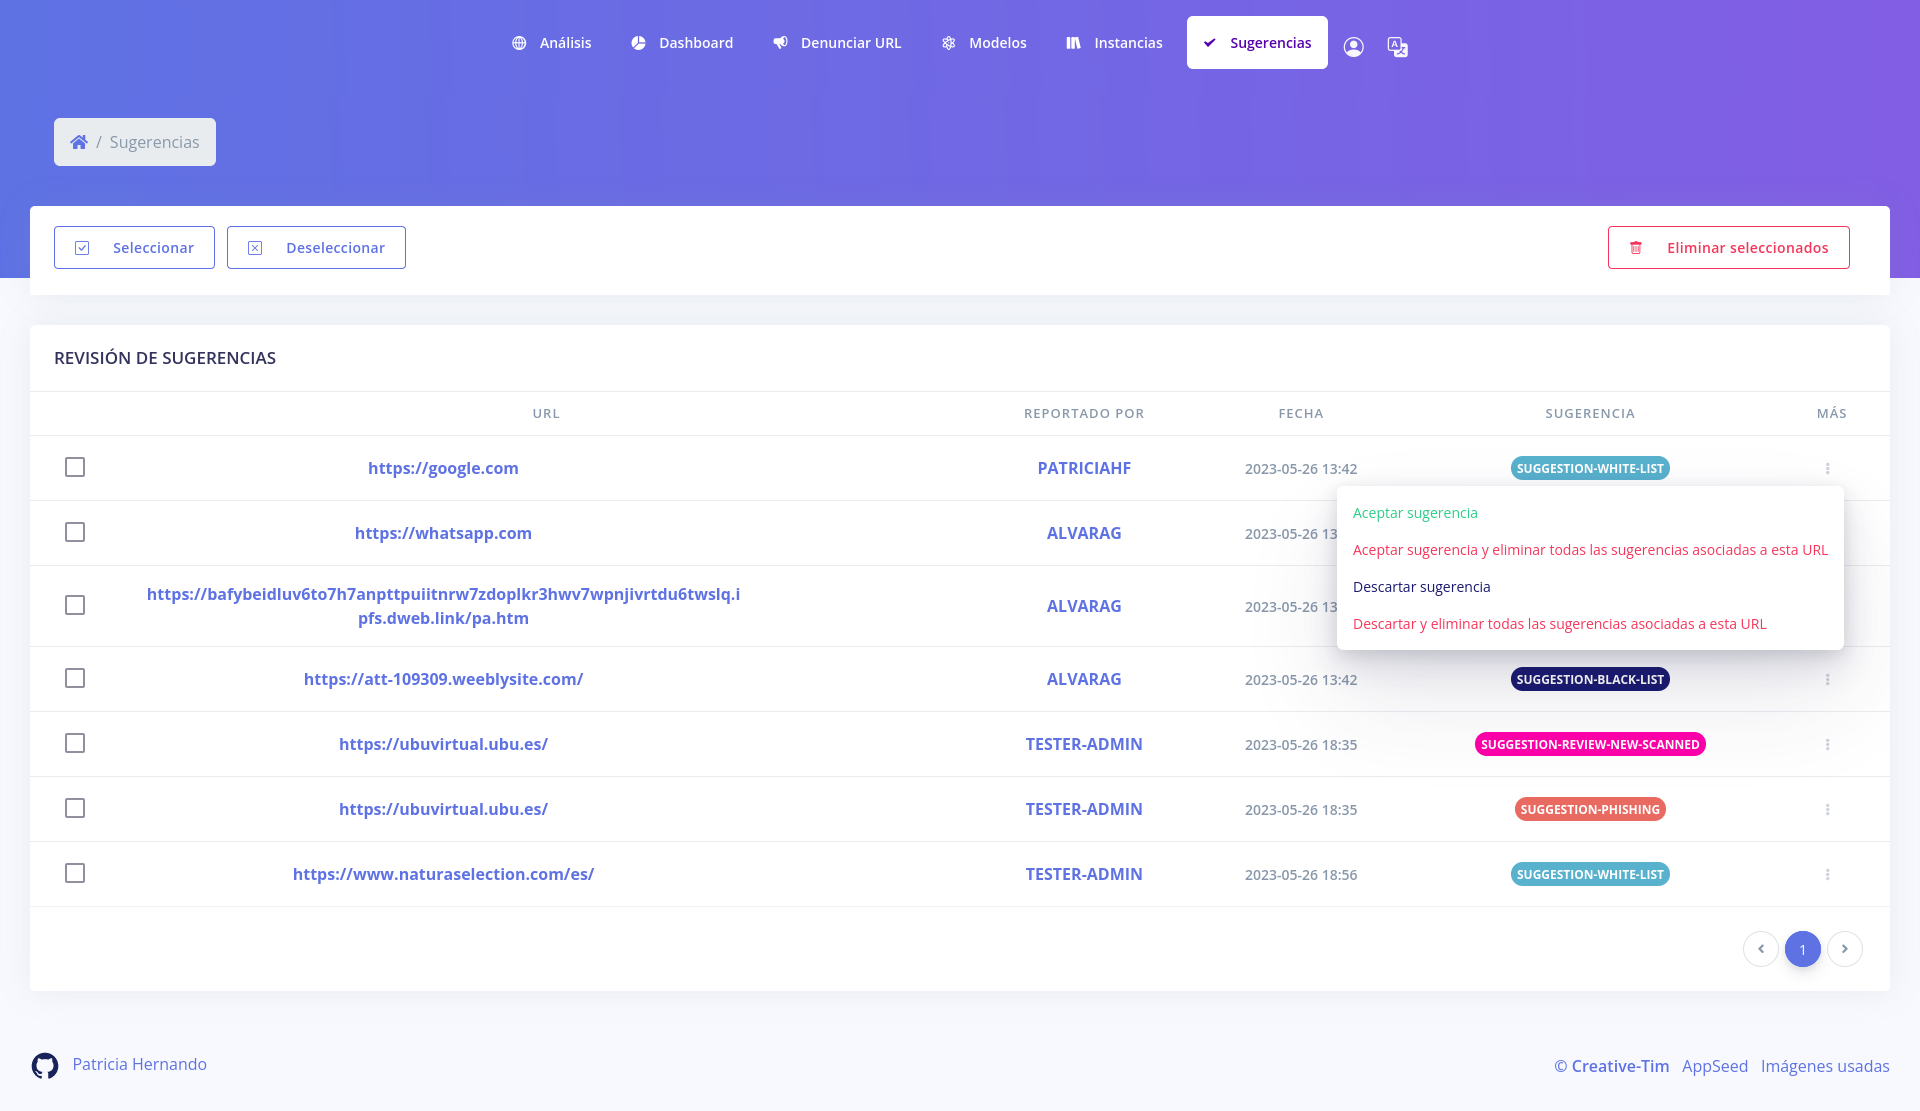
\includegraphics[width=\textwidth]{../img/anexos/user_guide/7_reports}
	\label{e-7:reports}
\end{figure}

Cada sugerencia realizada contiene una etiqueta en función del tipo, y se pueden aceptar o descartar pulsando en <<más>> (como se muestra en la imagen~\ref{e-7:reports}).

Aceptar una sugerencia implica que se modifica la URL afectada. Es decir, si se acepta una sugerencia que indica \texttt{suggestion-white-list}, la instancia pasará a ser marcada como perteneciente a una lista blanca. Si se acepta una sugerencia cuya etiqueta es~\texttt{suggestion-phishing}, la URL afectada se clasificará como \textit{phishing}, aunque fuese legítima anteriormente. Todas las etiquetas que presenten conflicto con el nuevo estado serán eliminadas.

\subsection{Usuarios, perfil, inicio de sesión y registro}

Cualquier usuario visitante podrá crear una cuenta (imagen~\ref{e-8:register}) e iniciar sesión en la \textit{web} (imagen~\ref{e-8:login}) proporcionando las credenciales que considere. Sin embargo, únicamente los administradores tendrán acceso a la funcionalidad completa de la aplicación\footnote{Para saber qué usuario puede realizar cada acción, consultar el diagrama de casos de uso~\ref{b:diagrama-cu}.}.

\begin{figure}[h]
	\caption[Manual de usuario: crear nueva cuenta]{Página de creación de nuevas cuentas.}
	\centering
	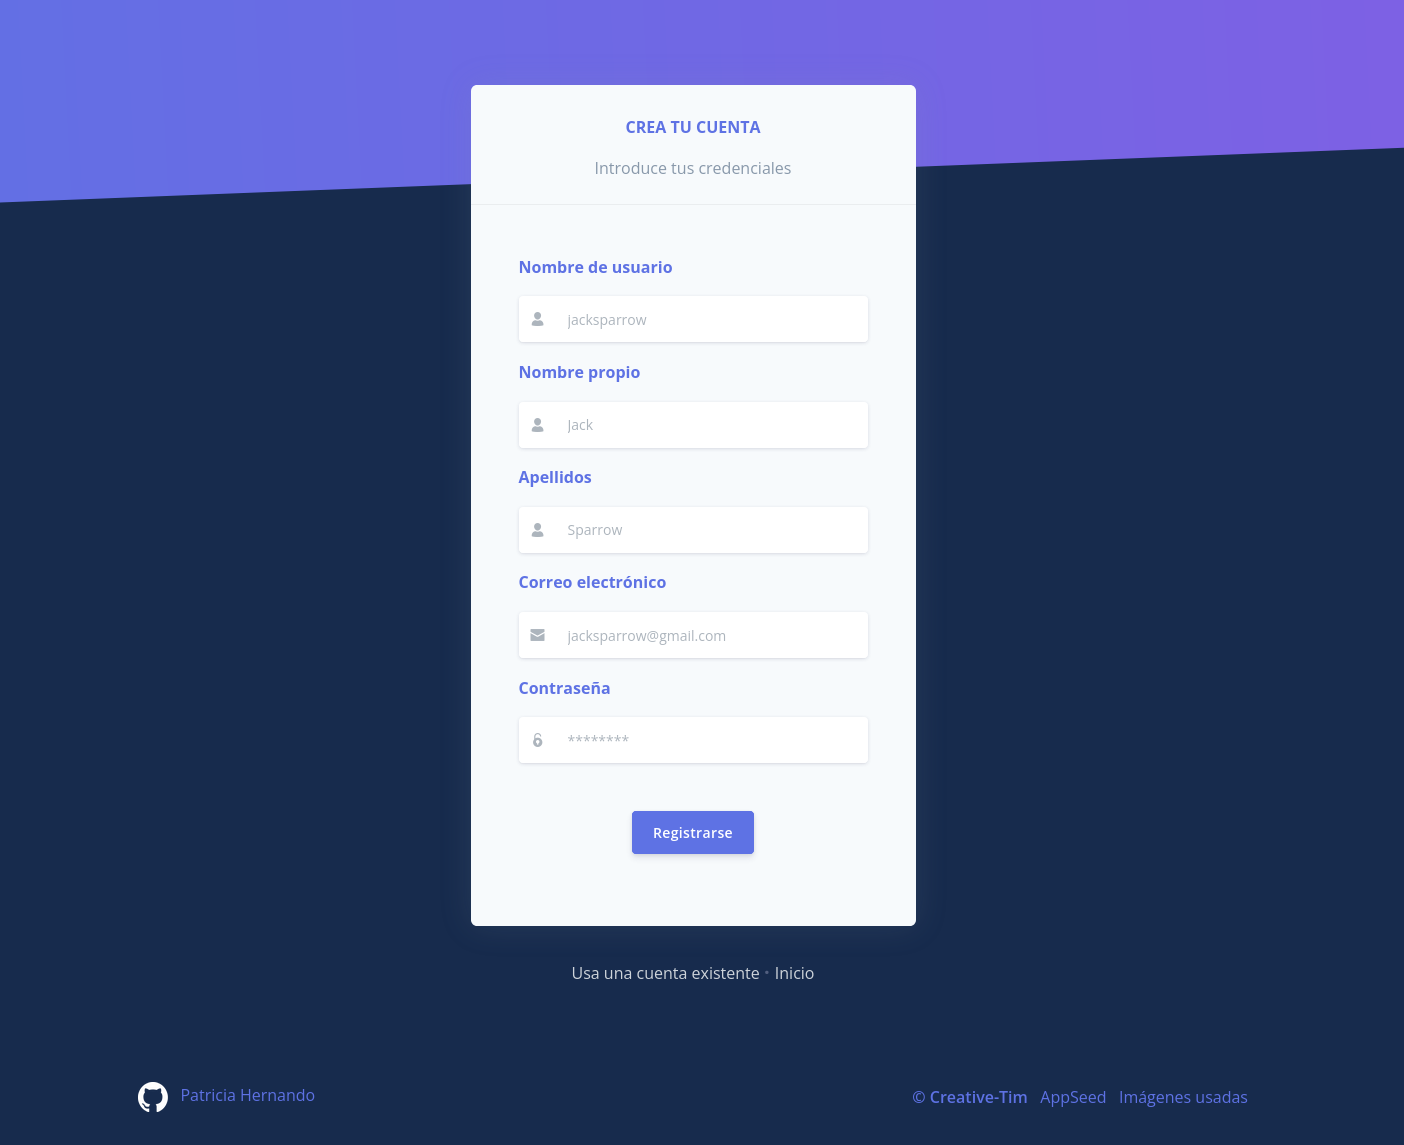
\includegraphics[width=\textwidth]{../img/anexos/user_guide/8_register}
	\label{e-8:register}
\end{figure}

\begin{figure}[h]
	\caption[Manual de usuario: inicio de sesión]{Página de inicio de sesión.}
	\centering
	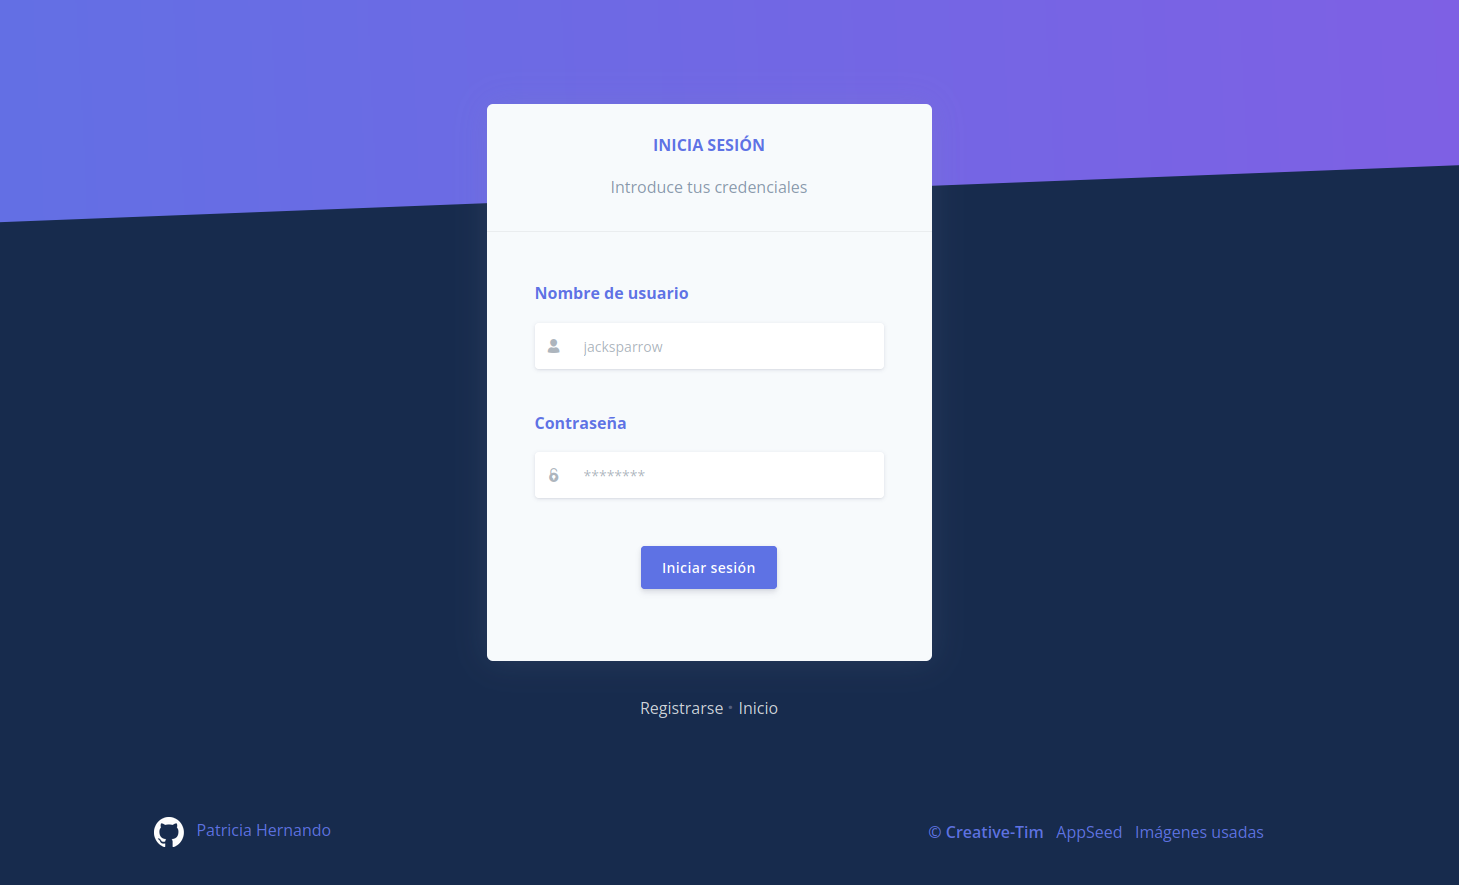
\includegraphics[width=\textwidth]{../img/anexos/user_guide/8_login}
	\label{e-8:login}
\end{figure}

Los usuarios registrados podrán, además, visualizar su perfil pulsando en el icono de usuario de la barra de navegación (consultar imagen~\ref{e-9:navbar}) y posteriormente en <<perfil>>. Esto renderizará la información correspondiente como se representa en la imagen~\ref{e-8:profile}, además de ciertas estadísticas como el número de URLs que el usuario ha denunciado que han sido aceptadas y el número de URLs que se encuentran en revisión.

\begin{figure}[h]
	\caption[Manual de usuario: perfil]{Perfil de un usuario que ha iniciado sesión en la aplicación.}
	\centering
	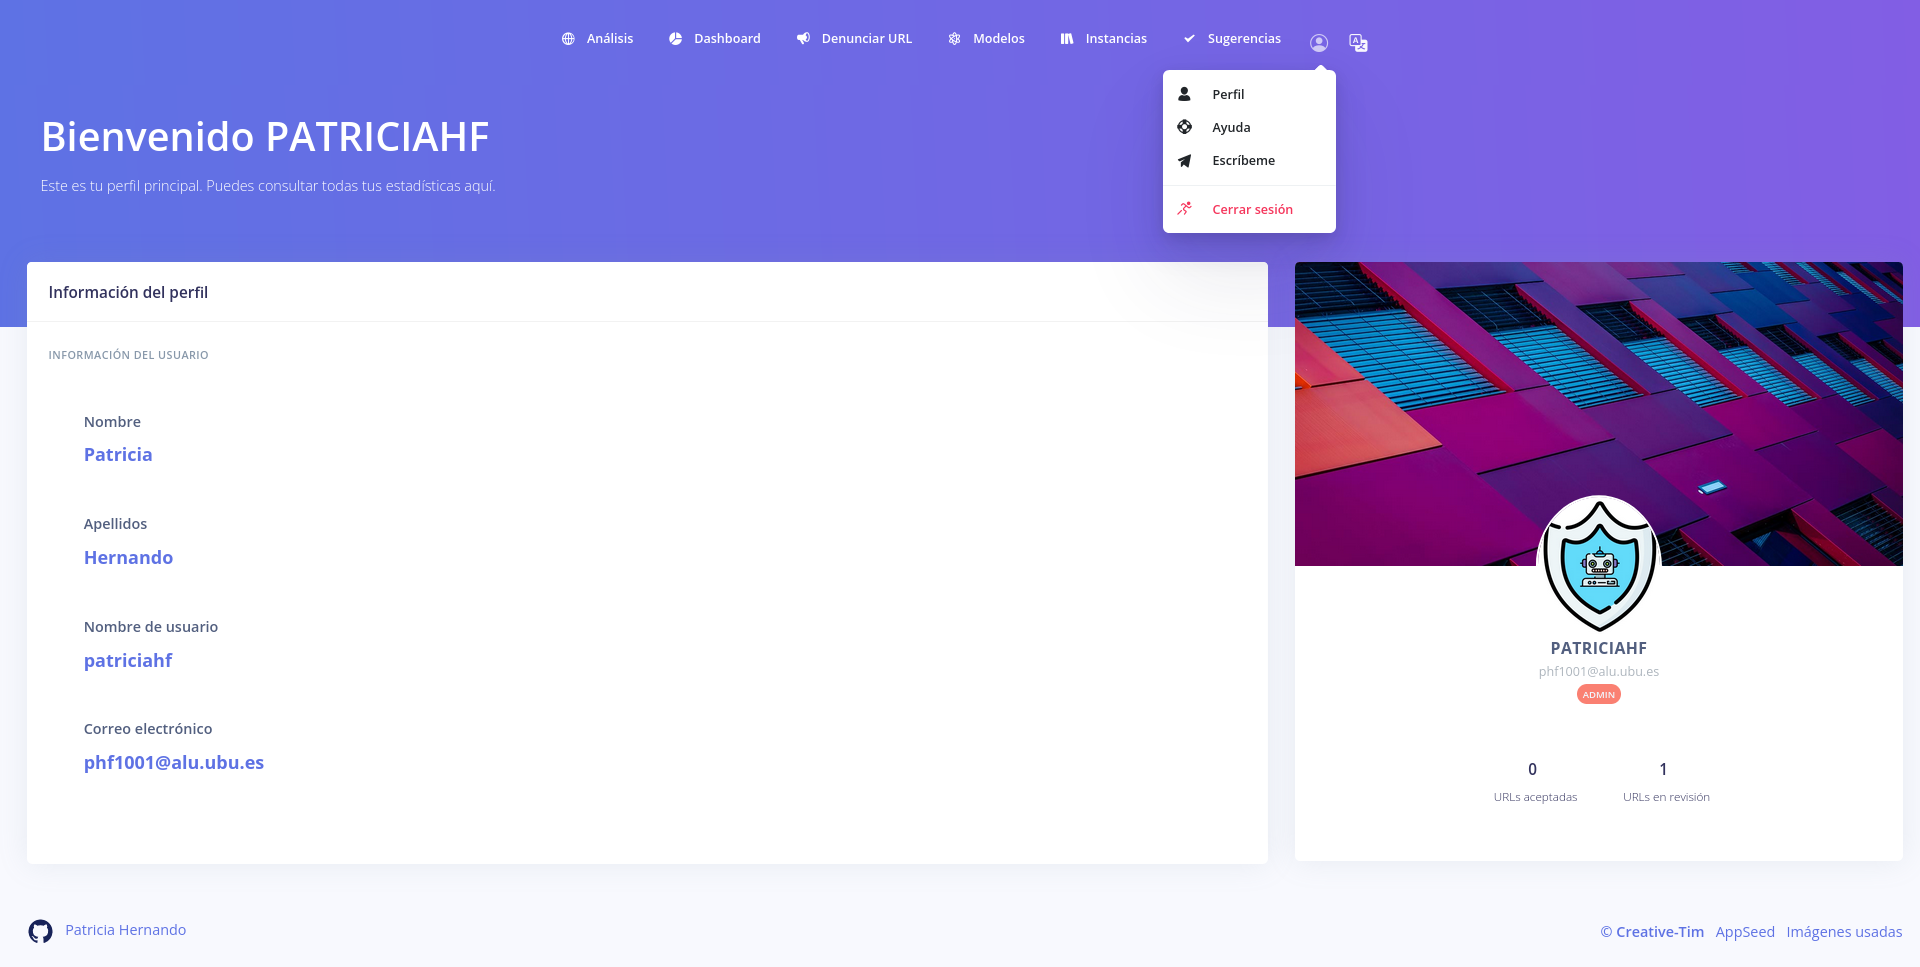
\includegraphics[width=\textwidth]{../img/anexos/user_guide/8_profile}
	\label{e-8:profile}
\end{figure}

Según los permisos que tenga el usuario, la barra de navegación mostrará unas funcionalidades u otras. El menú más sencillo corresponde a los usuarios visitantes y se muestra (con el menú de internacionalización desplegado) en la imagen~\ref{e-9:navbar-2}, mientras que la barra más compleja pertenece a los administradores y se muestra en la imagen~\ref{e-9:navbar} (con el menú de usuario desplegado).
\begin{figure}[h]
	\caption[Manual de usuario: barra navegación (usuario iniciado)]{Barra de navegación correspondiente a un administrador}
	\centering
	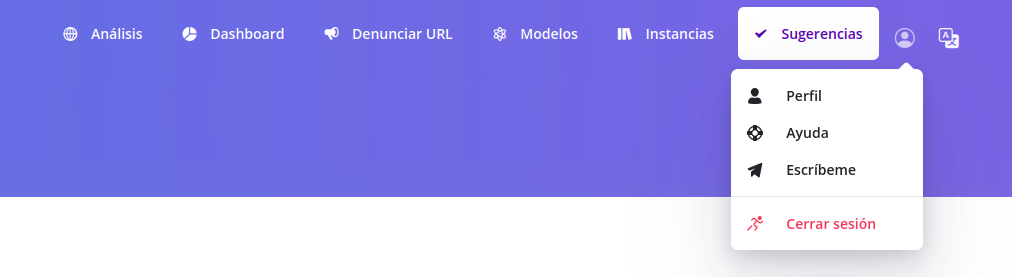
\includegraphics[width=\textwidth]{../img/anexos/user_guide/9_navbar_init}
	\label{e-9:navbar}
\end{figure}

\begin{figure}[h]
	\caption[Manual de usuario: barra navegación (visitante)]{Barra de navegación correspondiente a un usuario visitante.}
	\centering
	
\includegraphics[width=\textwidth]{../img/anexos/user_guide/9_navbar_no_init}
	\label{e-9:navbar-2}
\end{figure}


\subsection{Internacionalización}

Para cambiar el idioma de la aplicación, tan sólo se ha de pulsar en el icono correspondiente a idiomas en la barra de navegación. Esto abrirá un menú desplegable donde se podrá seleccionar el idioma deseado (consultar imagen~\ref{e-9:navbar-2}). Esta opción está disponible tanto para usuarios registrados como para visitantes.


\subsection{Pantallas de error}

Todos los errores que ocurran internamente son tratados para evitar que afecte a la experiencia del usuario. En caso de tratarse de excepciones, se mostrarán mensajes informativos adecuados. Por otro lado, los errores más graves tienen asociadas pantallas concretas (por supuesto, internacionalizadas) en función del tipo de código de error. Algunos ejemplos se muestran en las imágenes \ref{e-0:error-403}, \ref{e-0:error-404}, \ref{e-0:error-408} y~\ref{e-0:error-500}.

\begin{figure}[h]
	\caption[Manual de usuario: error 403]{Página de error 403.}
	\centering
	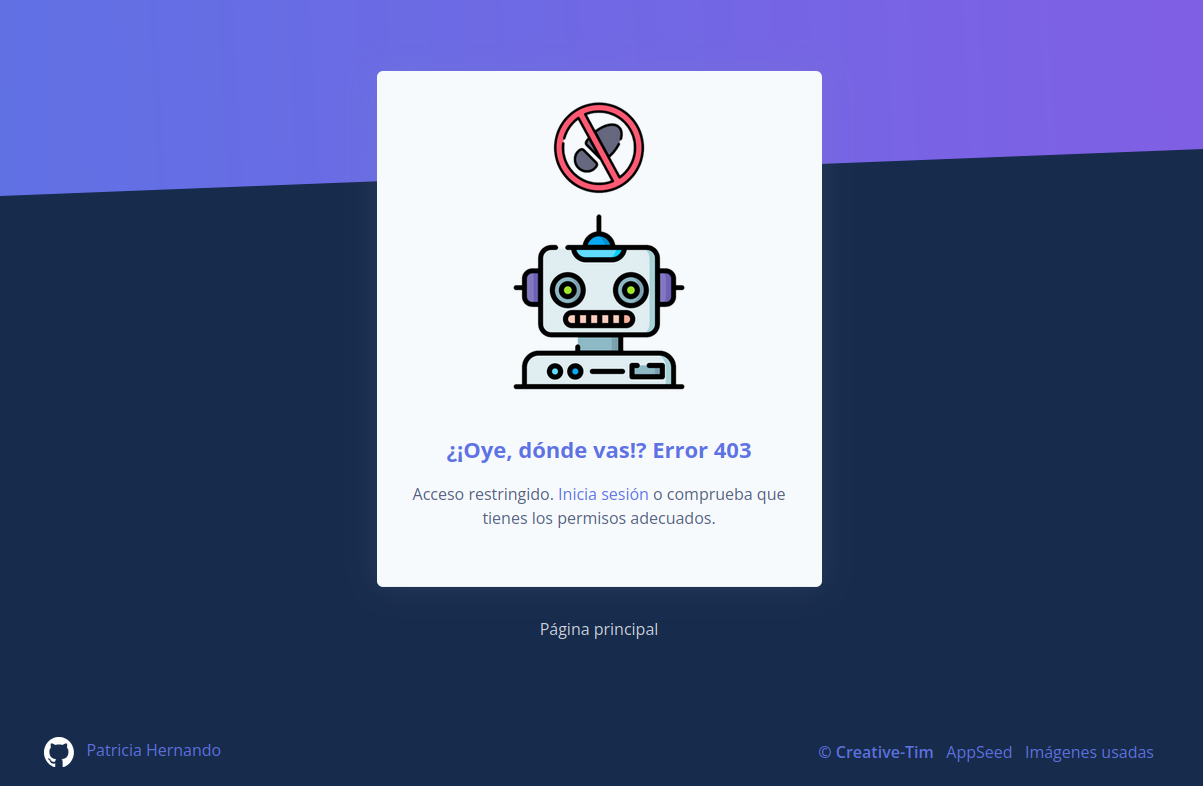
\includegraphics[width=\textwidth]{../img/anexos/user_guide/0_error_403}
	\label{e-0:error-403}
\end{figure}

\begin{figure}[h]
	\caption[Manual de usuario: error 404]{Página de error 404.}
	\centering
	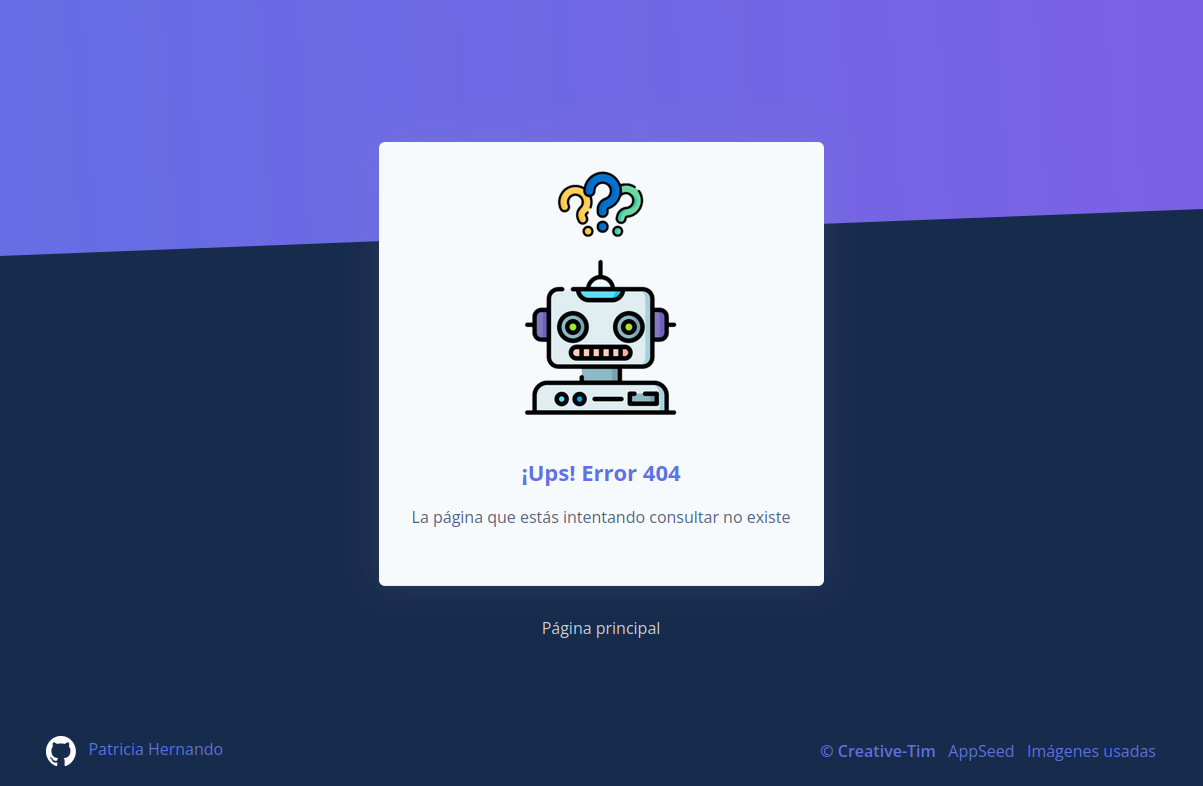
\includegraphics[width=\textwidth]{../img/anexos/user_guide/0_error_404}
	\label{e-0:error-404}
\end{figure}

\begin{figure}[h]
	\caption[Manual de usuario: error 408]{Página de error 408. Correspondiente a los \textit{timeouts} de Heroku.}
	\centering
	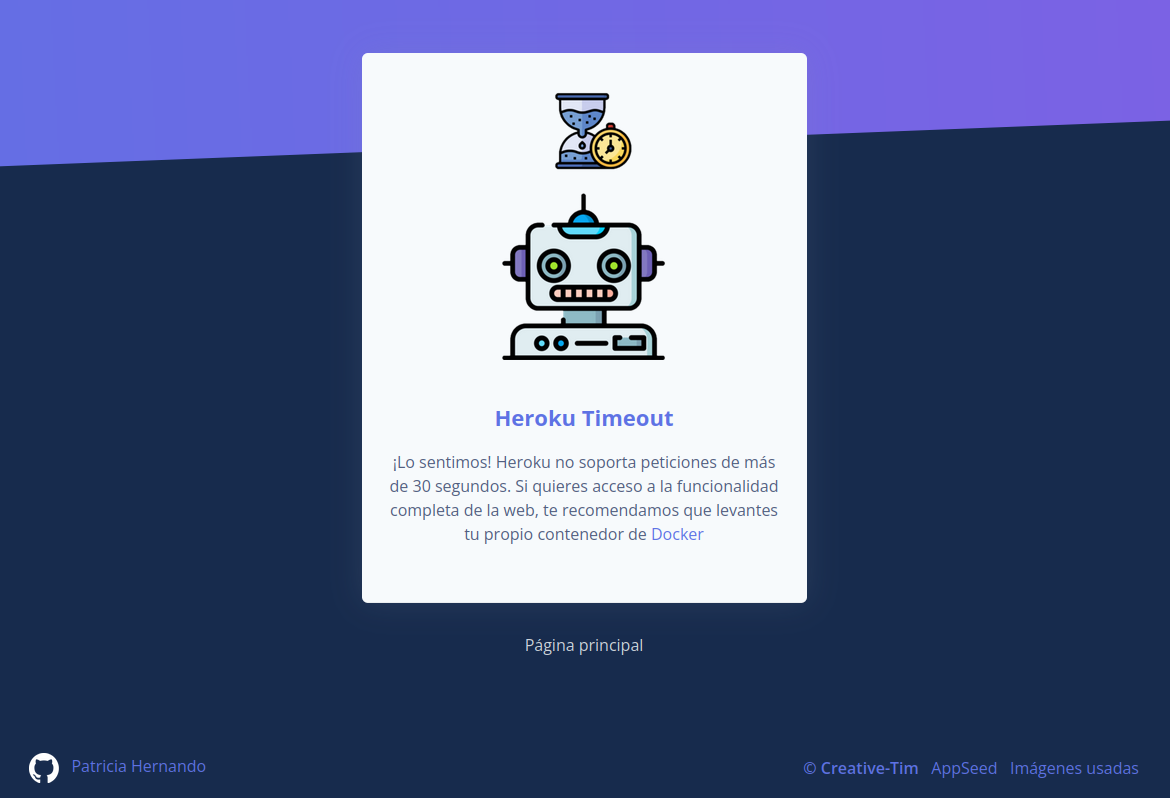
\includegraphics[width=\textwidth]{../img/anexos/user_guide/0_error_408}
	\label{e-0:error-408}
\end{figure}

\begin{figure}[h]
	\caption[Manual de usuario: error 500]{Página de error 500.}
	\centering
	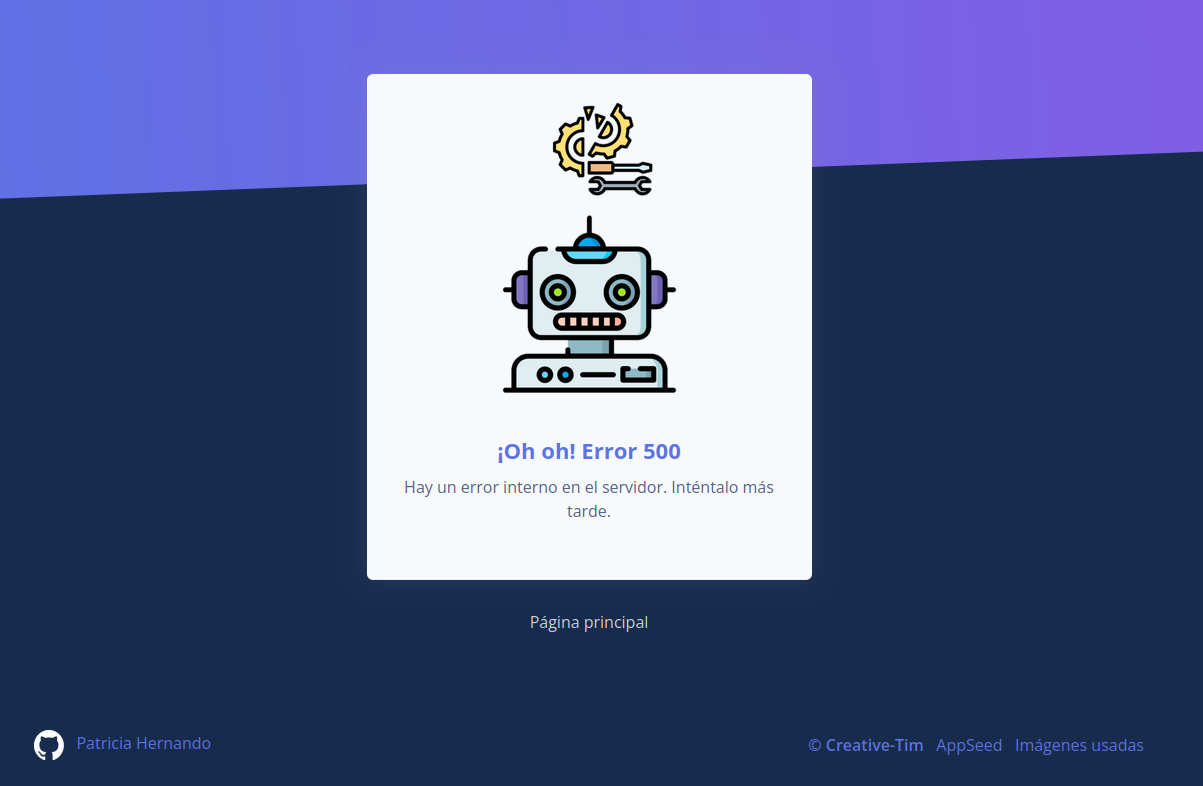
\includegraphics[width=\textwidth]{../img/anexos/user_guide/0_error_500}
	\label{e-0:error-500}
\end{figure}


\subsection{Responsividad y dispositivos móviles}

La página \textit{web} diseñada está adaptada para ser ejecutada en dispositivos móviles y para adaptarse a las medidas de las pantallas más pequeñas. Un ejemplo de como se visualiza el \textit{dashboard} en un dispositivo móvil se muestra en la imagen~\ref{e-0:dashboard-mobile}. La navegación, en este caso, se convierte en un menú <<hamburguesa>> (imagen~\ref{e-0:menu-mobile}).

\begin{figure}[h]
	\caption[Manual de usuario: \textit{dashboard} (versión móvil)]{\textit{Dashboard} visualizado desde el navegador de un teléfono.}
	\centering
	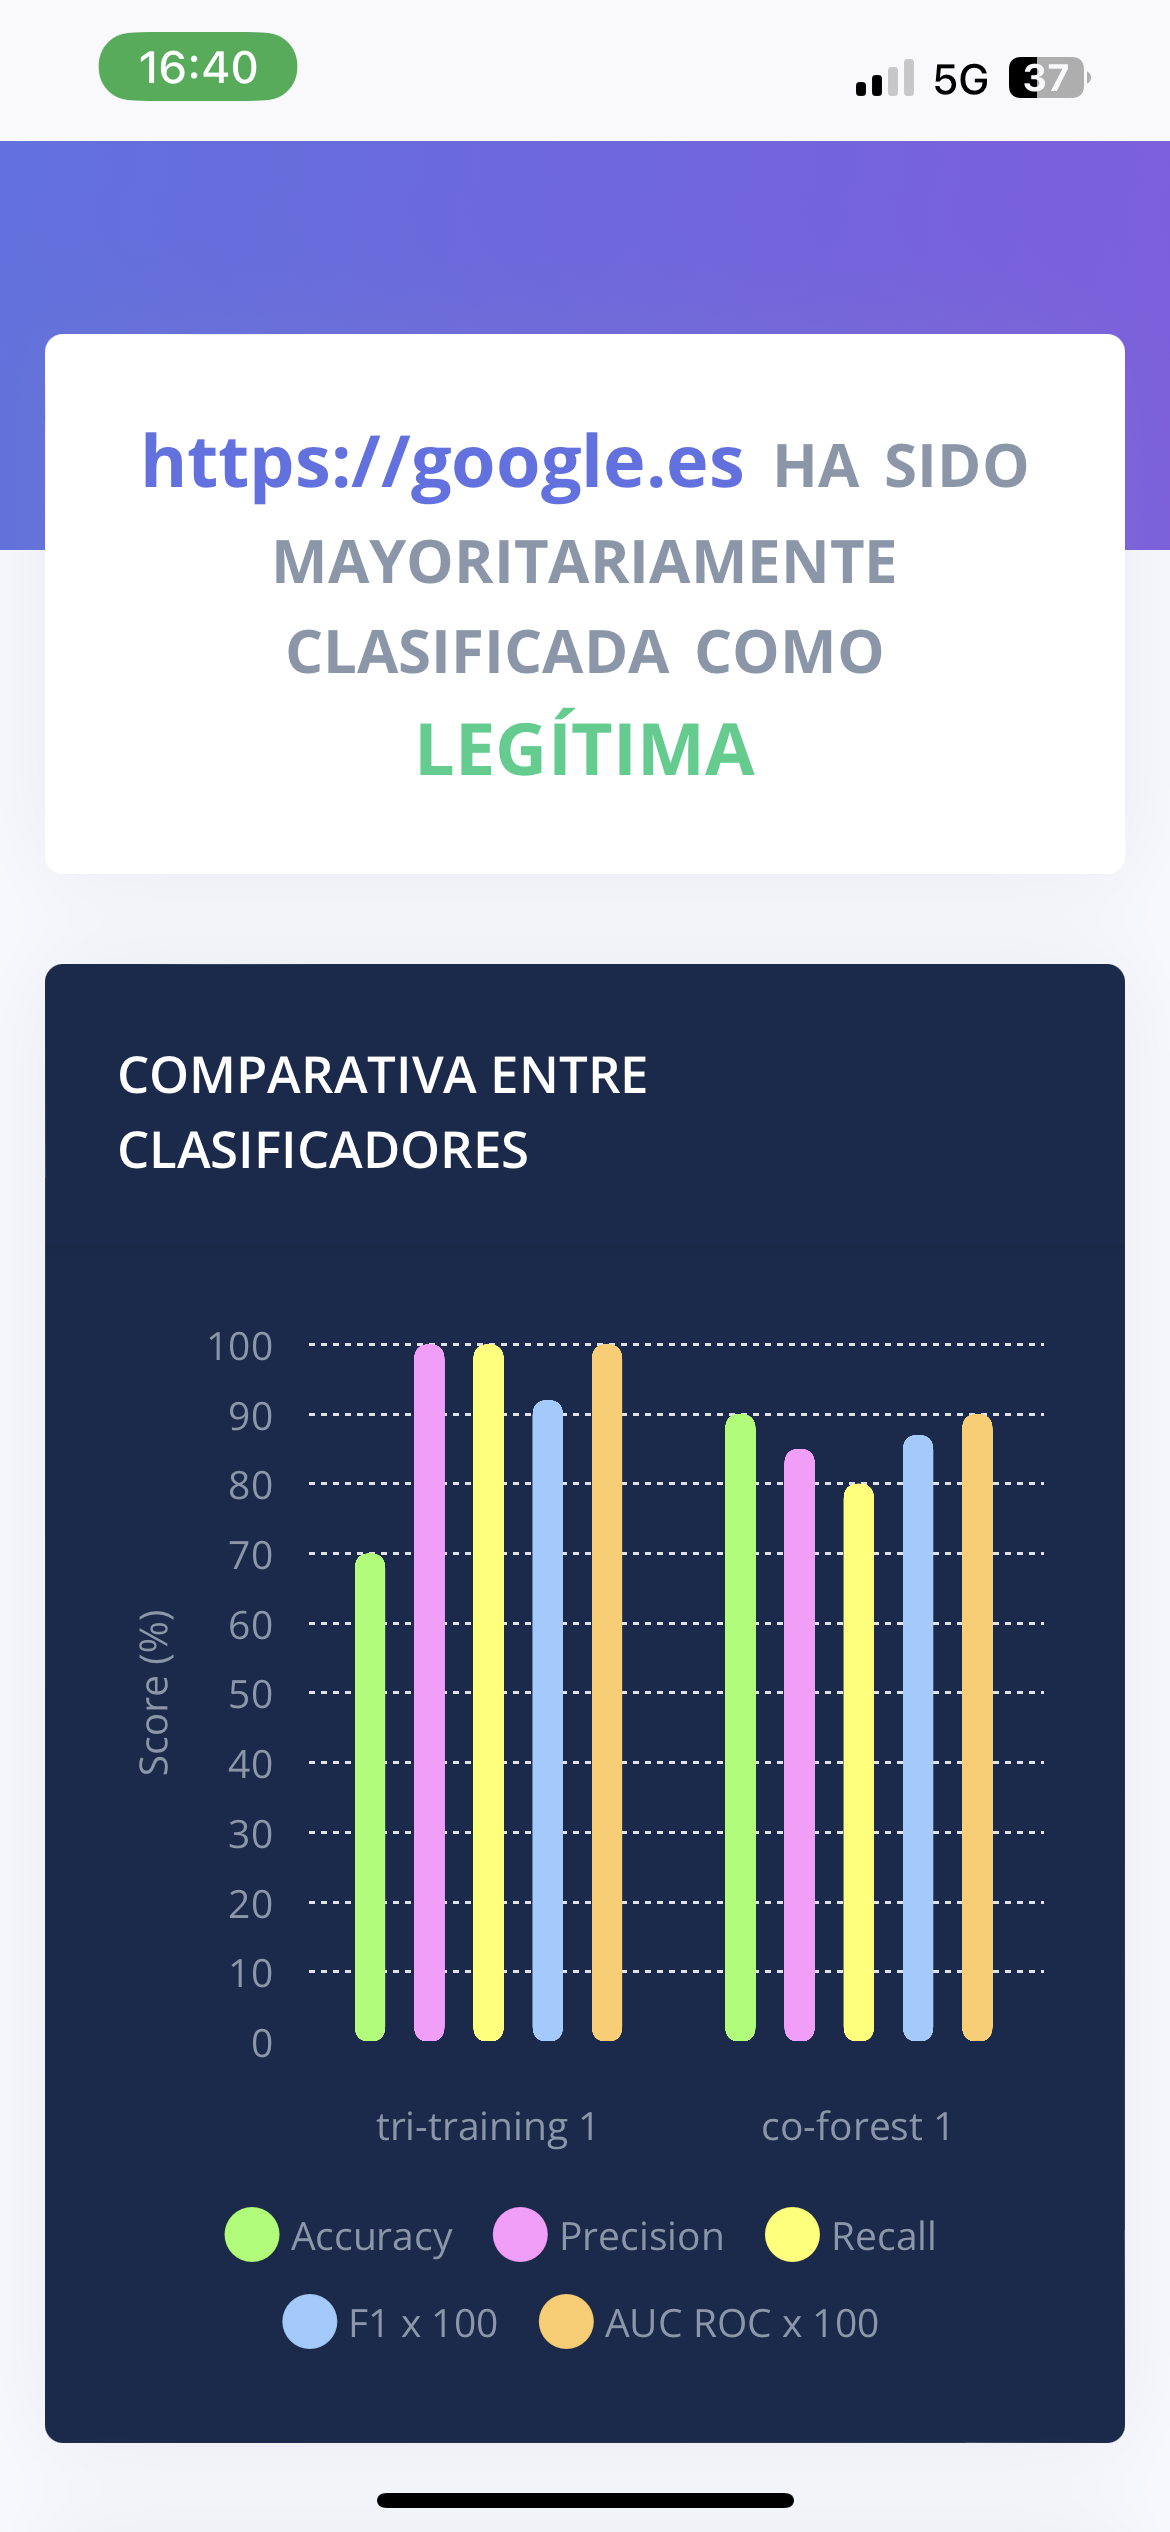
\includegraphics[scale=0.1]{../img/anexos/user_guide/0_dashboard_mobile}
	\label{e-0:dashboard-mobile}
\end{figure}

\begin{figure}[h]
	\caption[Manual de usuario: menú (versión móvil)]{Menú de navegación visualizado desde un dispositivo móvil.}
	\centering
	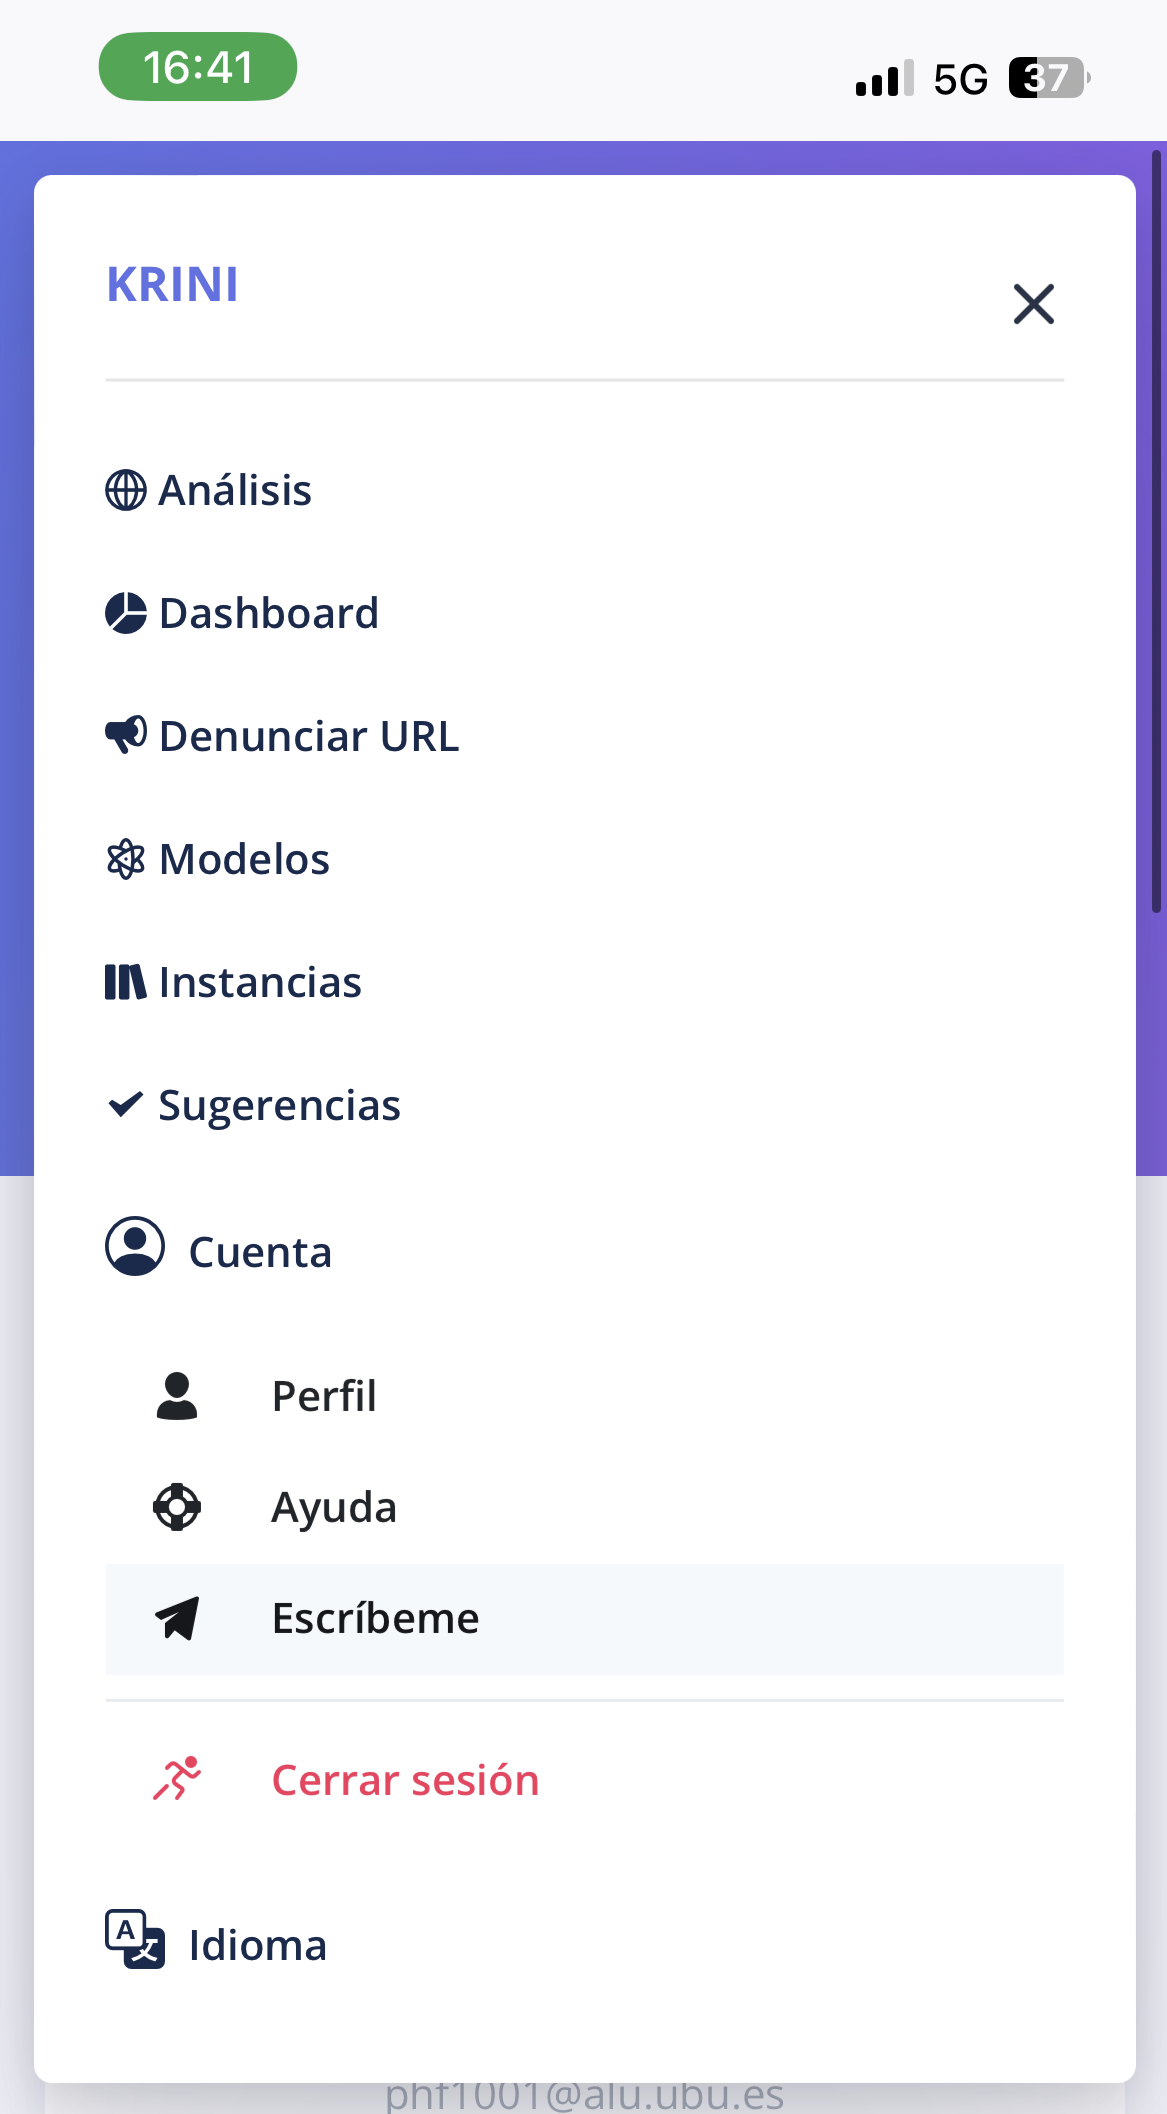
\includegraphics[scale=0.1]{../img/anexos/user_guide/0_menu_mobile}
	\label{e-0:menu-mobile}
\end{figure}